% Phương pháp tự đủ; trace dài được giữ trong kho bằng chứng.
\chapter{Proposed System}\label{s:9cf7f167cee0404f}
\section{System overview and one-decision walkthrough}\label{s:d04d6247a77e8f69}
At the end of an observed daily bar, the system summarizes the available
price and textual evidence, then proposes whether to enter the next LONG
cycle. Figure~\ref{fig:F03} separates offline fitting, deterministic
processing, hosted interpretation, external action policy and later
evaluation. The historical execution order is Indicator, Pattern, Trend,
then the joint alpha/sentiment stage. The figure groups computation types
rather than specifying that node order.

\begin{figure}[htbp]\centering
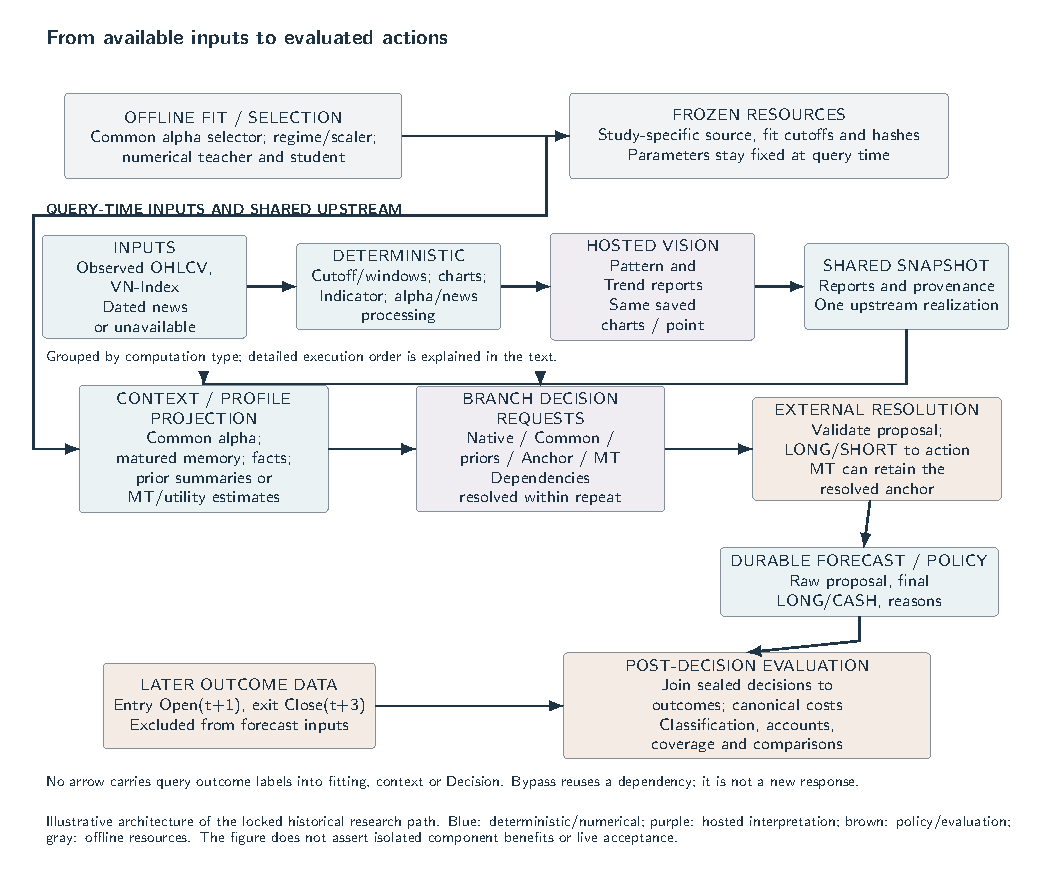
\includegraphics[width=\linewidth,height=.45\textheight,keepaspectratio]{../assets/diagrams/F03_system_overview.pdf}
\caption{The historical research path: frozen resources, shared reports,
context, hosted proposals and external policy. Query outcomes enter only
later evaluation. This is an architectural schematic, not a measured
benefit or evidence of live acceptance.}\label{fig:F03}
\end{figure}

Offline resources comprise the Common alpha selector, regime models and
scalers, and numerical teacher/student. Query inference does not refit
them. Indicator and numerical alpha processing are deterministic;
Pattern and Trend use hosted visual interpretation. Eligible Decision
branches obtain hosted responses, while documented bypasses reuse a
dependency. The numerical MT student is distinct from the hosted LLM.

One running case connects the stages: FPT at the \textbf{3 July 2023}
cutoff, upstream realization 0 and Decision repeat 0. Its 45-bar chart
and 600-bar prefix end at that cutoff; close is 48.18 in the stored price
unit, MACD is positive but below its signal, and close exceeds SMA20.
Verified news is unavailable. Entry/exit are scheduled for 4/6 July,
whose prices are withheld until the forecast path is complete. This is
a saved historical execution, not a trade shown to have occurred then.

\section{Input preparation and shared state}\label{s:26daba2236295e19}
The historical provider requires an exact cutoff and 600 clean
observations through it. It supplies the final 45 as chart/Indicator
input and the longer prefix to alpha. Pinned donor prices and separate
corporate-action event/barrier evidence retain their identities; the
barrier is not silently spliced into the donor series. VN-Index has its
own feature/calendar and fitted-resource identities. Historical news
uses the dated availability rule in Chapter 3; live crawler output is
not an interchangeable historical input.

Table~\ref{tab:contracts} gives the minimum interface needed to follow a
decision. Identity includes stock, cutoff, source and resource versions,
upstream realization and, later, Decision repeat. OHLCV arrays must align,
dates be ordered/unique, and the final row match the cutoff. Numbers
crossing the state boundary must be finite primitive JSON types or
explicitly unavailable; a missing value is not an observed zero.

\begin{table}[htbp]\centering\small\setstretch{1.05}
\caption{Compact input/output contracts. Temporal restrictions apply to
the underlying data, not only to the report's printed date.}\label{tab:contracts}
\begin{tabular}{@{}p{.20\linewidth}p{.38\linewidth}p{.35\linewidth}@{}}\toprule
Stage & Admissible input and processing & Output / absence contract\\\midrule
Preparation & Stock/date; pinned OHLCV and available news through cutoff & 45/600-row views; absent cutoff/history is an error\\
Shared analysis & Numeric inputs and saved chart images; no query target & Five reports, images/provenance; absence remains explicit\\
Historical context & Facts and mature history; frozen resources & Examples/statistics or marked tasks; support failure may bypass\\
Decision & Profile reports/context and same-repeat dependencies & Structured proposal or explicit reuse; failed calls remain failures\\
Policy/evaluation & Saved proposal and valid anchor; later outcome join & Final LONG/CASH, then labels/accounts; separate records\\\bottomrule
\end{tabular}\end{table}

The working graph accumulates intermediate fields; paired comparison uses
a narrower sealed snapshot with five report strings, query identity,
price prefix, optional images/projections and provenance. It is serialized
as immutable bytes; each branch decodes a fresh document, preventing
cross-branch mutation. The snapshot excludes the query label, future
entry/exit prices, realized return and Decision/prior material. Matured
historical labels enter through separate checked context interfaces.
Checksums bind identity and consistency, not economic authenticity or
row-wise causal validity.

\section{The base multi-agent pipeline}\label{s:b15ca1cf7b81c6ca}
\paragraph{Indicator.}
Python computes MACD, RSI, slow stochastic, Williams \%R and ROC using
the Chapter 3 settings. It applies priority-ordered heuristics and
aggregates bullish/bearish votes; MACD crossover rules precede histogram
rules. There is no extra historical LLM call for this role. Its numeric
table, categories and consensus feed shared reports and Decision. Warm-up,
nonfinite values and tool errors remain distinguishable from neutral
measurements. Correlated indicator votes are not independent trials.

\paragraph{Pattern and Trend.}
Pattern receives the 45-bar candlestick image, describing pattern,
confidence, bias, evidence, key candles and implication. A local OHLCV
check can flag conflict with recent candle bodies, including the last
five observations, and reduce confidence. It cannot validate every
pattern name or future prediction. Trend instead receives candles plus
fitted support/resistance geometry. Its colored boundaries are fitted
to Close values using residual pivots and constrained slopes; additional
high/low fits are separate. It returns direction, levels, slope, price
relation, explanation and forecast. A direction/price-summary verifier
does not certify every level or geometric assertion. Formatting and text
fallback paths retain their execution provenance.

The FPT case illustrates their distinction. The saved Pattern report
has low-confidence upward bias and retains a contradiction warning:
four of the final five candles close below their opens. Trend reports
upward direction and high confidence, support 47.8 and resistance 49.2.
Its widening-channel claim disagrees with the saved-input geometric
check: the colored Close-line gap decreases from 1.885784 to 1.456185
price units. Those named levels are not the exact fitted endpoints.
These are presentation summaries of stored reports, not new forecasts.
Suggested stops/pullbacks in prose do not replace the fixed execution
contract. The two chart views carry different information despite
sharing the same underlying bars.

\paragraph{Alpha.}
The registry has 85 candidates: five system-specific factors and 80
single-stock Alpha101 adaptations. The price proxy $(H+L+C)/3$ is not
observed VWAP, and temporal ranks do not recreate cross-stock ranks.
\autocite{kakushadze2016formulaic} Native evaluates candidates on at most
600 cutoff-limited rows, with full-window normalization and IC-based
orientation. Its default score combines normalized absolute Spearman IC,
accuracy and diagnostic Sharpe with weights .40/.35/.25; the top five
feed its report. Its symmetric sign-return diagnostic is a ranking
device, not the LONG/CASH account payoff. Latest oriented values above
.10 or below $-.10$ become bullish/bearish, with neutral boundaries.
In-sample selection and whole-window transformations mean that an outer
cutoff does not certify historical feature causality.

Common replaces affected operations with expanding-prefix normalization,
lags without backward filling, observed volume and fixed versions of six
length-dependent expressions. A 300-bar volume mask, 20-observation
normalizer minimum and finite-value requirements determine availability.
Train Spearman IC fixes orientation; validation selects five factors and
one threshold from .05/.10/.20 by LONG/CASH return on common finite
support. Minimums are 60 train pairs, 30 validation observations and five
LONGs per admitted candidate. Alpha-ID ties and the smaller threshold
resolve equal scores. Three-session grids and strict maturity separate
splits. IDs/signs/threshold are frozen; prediction does not reselect.
Unavailable selected query factors raise errors rather than being filled
or substituted. This scoped Common repair does not certify the whole
system, and Native's recorded row-wise gate remains FAIL.

\paragraph{Sentiment.}
The live agent collects CafeF title/snippet text, checks company relevance
and records backend/fallback provenance. The configured ViSoBERT-based
three-label classifier uses signed confidence; lexicon fallback uses a
different keyword score. Historical adapters consume frozen aggregates
or verified dated scores instead. The context study uses the 90-day,
three-score, 30-day-half-life rule; missingness cannot become neutral
financial evidence. Alpha and sentiment are produced together in the
graph but summarize different sources. No new article collection or
classifier validation is implied by this integration.

\paragraph{Decision.}
The request prioritizes Trend/Pattern for direction/timing, Indicator for
momentum, Alpha for numerical evidence and sentiment last. The LLM
synthesizes condensed reports rather than recalculating them. Structured
output contains LONG/SHORT, horizon, textual confidence, risk--reward
ratio in $[1,5]$, evidence and justification. Confidence and risk--reward
are report claims, not calibrated probabilities or executable orders.
The external resolver maps SHORT to CASH and can retain an anchor after
inspecting a proposal. Schema/transport failure cannot silently create
a valid SHORT/CASH result.

\section{Native and Common foundations}\label{s:34c72d872d464412}
The context study's Native uses the recorded native serving factory,
alpha report and compact request. Common starts from the same sealed
parent, preserving images, Indicator/Pattern/Trend, sentiment and price
prefix while replacing the top-level alpha projection with its verified
causal-common profile. Raw Native fields remain available for provenance.
Common also changes report caps and instructions: prior/target/query
notation, probability versus utility and SHORT=CASH are explicit. Common
itself supplies an \emph{empty} history prefix; mentioning task notation
does not create context. The shared serving envelope fixes point/repeat,
model/options and schema, not identical prompt content.

The separate component study compares Full, enabling alpha and sentiment,
with Base, omitting their joint bundle. Indicator--Pattern--Trend run once
and are deep-copied to both branches. Full/Base therefore changes both
information and prompt representation. It is not Native/Common and does
not isolate Alpha or Sentiment alone. Likewise, a Native/Common bridge
cannot attribute a difference solely to normalization, instructions or
context; several ingredients change together. Extensions below reuse
the same-repeat Common result when their documented support gate fails.

\section{Historical memory and market regimes}\label{s:caa6b0b420cdae1c}

Historical evidence has two representations. Signal memory stores completed
trading cycles with categorical agent conclusions. Numerical MT context
groups price-derived observations into tasks. Both require mature labels,
but they have different fields, membership rules and sources; a count of
signal examples cannot be substituted for a count of tasks or observations.

\subsection{A completed signal episode}\label{s:f56f0c52fd4c64ea}

A signal episode contains an ID, stock, decision/entry/exit dates, a regime
label, five agent signals and the candidate-LONG outcome. Signals describe
what the agents concluded at the historical decision; the outcome describes
what subsequently happened under the fixed economic contract. A bullish
signal is not retrospectively changed to bearish because the trade lost.
\footnote{SYS19 \texttt{bayesian\_\allowbreak{}memory}, TIME01 economic oracle, and the frozen HistoricalTaskRecord schema; CL055--CL056 in ledger §9.9. The saved example is joined by ID to both the original bank and the U08 retrieval trace, not reconstructed from a model narrative.}

\begingroup
\small
\setstretch{1.05}
\setlength{\tabcolsep}{3pt}

\begin{longtable}[]{@{}
  >{\raggedright\arraybackslash}p{(\linewidth - 2\tabcolsep) * \real{0.3000}}
  >{\raggedright\arraybackslash}p{(\linewidth - 2\tabcolsep) * \real{0.7000}}@{}}
\caption{A completed signal episode - supporting detail}\label{tab:04_proposed_system:7}\tabularnewline
\toprule\noalign{}
Field group
 & Meaning and validation
 \\
\midrule\noalign{}
\endfirsthead
\toprule\noalign{}
Field group
 & Meaning and validation
 \\
\midrule\noalign{}
\endhead
\bottomrule\noalign{}
\endlastfoot
\texttt{episode\_\allowbreak{}id}, \texttt{symbol} & Stable identity and admitted stock; duplicate IDs or duplicate stock/decision cycles are rejected. \\
\texttt{as\_\allowbreak{}of\_\allowbreak{}date}, \texttt{entry\_\allowbreak{}date}, \texttt{exit\_\allowbreak{}date} & Exact ISO dates on the source's observed-session calendar: decision, next open, third future close. Dates must increase and execution-price/event checks must admit the cycle. \\
\texttt{regime} & Stored category BULL, BEAR, CHOPPY or CONSOLIDATION; it is not the candidate trade's future label. \\
\texttt{agent\_\allowbreak{}signals} & Nonempty \texttt{trend}, \texttt{pattern}, \texttt{alpha\_\allowbreak{}consensus}, \texttt{indicator\_\allowbreak{}consensus}, \texttt{sentiment}; retrieval additionally validates declared aliases instead of searching arbitrary prose for a direction. \\
\texttt{outcome} & Finite \texttt{net\_\allowbreak{}return\_\allowbreak{}pct}, UP/\allowbreak{}DOWN, WIN\_\allowbreak{}IF\_\allowbreak{}LONG/LOSS\_\allowbreak{}IF\_\allowbreak{}LONG, and Boolean \texttt{was\_\allowbreak{}bull\_\allowbreak{}trap}; all must agree with canonical execution arithmetic. \\
\end{longtable}

\endgroup

The memory validator obtains the admissible entry/exit prices and calls
\texttt{compute\_\allowbreak{}round\_\allowbreak{}trip\_\allowbreak{}net\_\allowbreak{}return}, then expresses its result as a percentage.
UP and WIN\_\allowbreak{}IF\_\allowbreak{}LONG require a strictly positive return; nonpositive values,
including zero, are DOWN and LOSS\_\allowbreak{}IF\_\allowbreak{}LONG. Bull trap means that at least one
of Trend or Pattern was bullish while the candidate LONG return was
nonpositive. It is a retrospective label of this convention, not proof of
market manipulation. LOSS\_\allowbreak{}IF\_\allowbreak{}LONG does not mean that a CASH action lost
money. The loader rejects missing/extra fields, invalid dates/types,
inconsistent economics, duplicate cycles and overlapping holding intervals
for a stock; it does not silently repair a malformed bank.

\textbf{Saved record example.} The first EX01 signal example is reproduced with
its original field names and numerical precision:

\begin{Verbatim}[fontsize=\small,breaklines=true,breakanywhere=true]
{
  "episode_id": "FPT:2022-04-07",
  "symbol": "FPT",
  "as_of_date": "2022-04-07",
  "entry_date": "2022-04-08",
  "exit_date": "2022-04-13",
  "regime": "CONSOLIDATION",
  "agent_signals": {
    "trend": "BULLISH",
    "pattern": "BULLISH",
    "indicator_consensus": "BEARISH",
    "alpha_consensus": "BULLISH",
    "sentiment": "NEUTRAL"
  },
  "outcome": {
    "actual_direction": "UP",
    "net_return_pct": 0.8800636494421088,
    "was_bull_trap": false,
    "result": "WIN_IF_LONG"
  }
}
\end{Verbatim}

The sentiment code preserves the bank's categorical representation. It does
not establish that reliable news existed for this record, or replace the
query's unavailable news. The bank's recorded sentiment-reliability coverage
remains a separate limitation.

\subsection{Temporal eligibility and frozen membership}\label{s:885d13890b35232b}

An episode can be a historical observation at cutoff \(t\) only when its
exit is \textbf{strictly before} \(t\). A decision date before \(t\) is insufficient
if the holding interval still crosses \(t\). Outcomes may be aggregated only
after this maturity filter; the query's outcome remains outside forecast
inputs. Memory returns independent copies of eligible records so a branch
cannot mutate another branch's evidence.

\begingroup
\small
\setstretch{1.05}
\setlength{\tabcolsep}{3pt}

\begin{longtable}[]{@{}
  >{\raggedright\arraybackslash}p{(\linewidth - 4\tabcolsep) * \real{0.2400}}
  >{\raggedright\arraybackslash}p{(\linewidth - 4\tabcolsep) * \real{0.3900}}
  >{\raggedright\arraybackslash}p{(\linewidth - 4\tabcolsep) * \real{0.3700}}@{}}
\caption{Temporal eligibility and frozen membership - supporting detail}\label{tab:04_proposed_system:8}\tabularnewline
\toprule\noalign{}
Timeline example at EX01 cutoff 3 July 2023
 & Decision \ensuremath{\rightarrow} entry \ensuremath{\rightarrow} exit
 & Eligibility
 \\
\midrule\noalign{}
\endfirsthead
\toprule\noalign{}
Timeline example at EX01 cutoff 3 July 2023
 & Decision \ensuremath{\rightarrow} entry \ensuremath{\rightarrow} exit
 & Eligibility
 \\
\midrule\noalign{}
\endhead
\bottomrule\noalign{}
\endlastfoot
Saved \texttt{FPT:\allowbreak{}2022-\allowbreak{}04-\allowbreak{}07} & 7 April \ensuremath{\rightarrow} 8 April \ensuremath{\rightarrow} 13 April 2022 & Mature: exit precedes cutoff. \\
Saved \texttt{FPT:\allowbreak{}2022-\allowbreak{}04-\allowbreak{}13} & 13 April \ensuremath{\rightarrow} 14 April \ensuremath{\rightarrow} 18 April 2022 & Mature, although its candidate LONG lost. Eligibility does not depend on winning. \\
Saved \texttt{FPT:\allowbreak{}2022-\allowbreak{}04-\allowbreak{}18} & 18 April \ensuremath{\rightarrow} 19 April \ensuremath{\rightarrow} 21 April 2022 & Mature, with a stored bullish-trap label. \\
\textbf{Illustrative boundary}, not an archived episode & Any earlier decision with exit on 3 July 2023 & Excluded: equality is not strict precedence. \\
\textbf{Illustrative boundary}, not an archived episode & Any earlier decision with exit after 3 July 2023 & Excluded: outcome is not yet admissible. \\
\end{longtable}

\endgroup

The evaluated signal bank contains 852 completed records for FPT, MWG, VCB
and VNM, with the latest exit on 30 December 2022. Its manifest and published
QA bind the records, schema and provenance. The context-study adapter reuses
this frozen bank; it does not append later query outcomes or manufacture
same-stock memory for the other five query stocks. Source prices used to
validate bank labels differ from the query vendor series. This explicit
transfer is retained, including recorded label-basis discrepancies; the
bank is not relabeled using query prices to make the sources appear equal.
Published QA and normalized signals do not imply a newly recovered raw
signal-call journal.\footnote{SYS21 \texttt{free\_\allowbreak{}pilot\_\allowbreak{}assets.\allowbreak{}FrozenBank}, BG16 \texttt{FrozenStudyBank/\allowbreak{}FrozenStudyStream}, BG17 execution-provider freeze, SYS20 historical signal adapter and BG23 context gates. CL057--CL058 preserve CORE4 membership, raw-bank/query transfer, reserved IDs and numerical-context distinctions.}

Numerical MT context is separately frozen before the first query of a fold.
Its observation stream admits only exits before that boundary, and all
102 reserved evaluation IDs are withheld before historical labels can enter
context construction. Later queries can have new unlabeled features while
the fold's admitted labeled history remains fixed. This is stricter than
simply appending every cycle that has become mature by each later query.
The fitted scaler and its membership are separate frozen resources.

\subsection{Signal memory versus numerical context in EX01}\label{s:e3dc0a930725f6dc}

EX01's signal retrieval starts from 211 admissible FPT records, with 19 in
the requested regime and at most three displayed examples. The three saved
IDs in the timeline belong to that signal bank. The numerical context
instead has three prior tasks containing 11 observations and three target
observations: 14 labeled historical rows in total. Its query belongs to
the target task but has no \texttt{y} or realized return in the context. These
groups are not the three signal episodes above; task construction and
numerical feature scaling are detailed in Section 4.8.

Signal memory's CONSOLIDATION and numerical context's BULL also come from
different regime resources. Their provenance is explained next; the labels
must not be silently unified for this example. IDs, sources and membership
checks establish traceability, while frozen-resource integrity alone cannot
certify the validity of every historical signal or hosted-model training
exposure.

\subsection{Regime fitting and query-time assignment}\label{s:0c387f2c106e9338}

Regime is a description of the market state used to organize historical
evidence. It is computed from VN-Index, not from the query's eventual trade
outcome. The feature definitions and HMM interpretation were introduced in
Section 3.4. Here the important distinction is between \textbf{fitting a resource}
and applying an already frozen resource to the admissible query prefix.
\footnote{BG04 \texttt{regime\_\allowbreak{}detector}, SYS22 \texttt{historical\_\allowbreak{}evaluation\_\allowbreak{}runner.\allowbreak{}Regimes}, SYS23 \texttt{mt\_\allowbreak{}bicl\_\allowbreak{}regimes.\allowbreak{}RegimeTimeline}, BG23 \texttt{hydrate/\allowbreak{}FrozenTimeline}, and SYS24 historical prefix provider. CL059--CL061 and ledger §9.10 bind settings, mapping, fallback and the absence of query-time fitting.}

\textbf{Offline fitting and naming.} The primitive constructs five features:
log return, 20-session return volatility and relative distances to the
20/50/200-session moving averages. It needs 200 observed sessions for the
longest moving average and at least 300 feature rows to fit. A train-only
StandardScaler feeds a four-state diagonal Gaussian HMM. The configured
seed is 42, iteration ceiling 500, convergence tolerance 0.001 and minimum
covariance 0.001. These settings describe the evaluated implementation;
the effective date range comes from each artifact, not the generic
2018--2022 fitting bounds in the class.

Latent state numbers have no intrinsic BULL/BEAR meaning. Train posterior
weights produce state feature means and occupancies. The highest mean
distance to MA200 names BULL, the lowest remaining mean names BEAR, and the
higher-volatility state among the two remaining states names CHOPPY. The
last state names CONSOLIDATION; deterministic state-index tie-breaking makes
the mapping reproducible. Mapping and calibration are stored with the
model, scaler, source/runtime versions and training-data hash.

\textbf{Fit-quality fallback.} The primitive checks its registered EM convergence
criterion, posterior occupancy of at least 5\% per state, BULL/BEAR means on
opposite sides of MA200, sufficient separation relative to train MA200
dispersion, and a CHOPPY volatility mean at least 1.1 times the remaining
neutral state's mean. If a check fails, metadata records reasons and sets
\texttt{classification\_\allowbreak{}method=MULTI\_\allowbreak{}FACTOR}. The deterministic fallback uses
MA50/MA200 distances with a train-derived trend threshold, followed by an
upper-train-volatility-quantile rule; otherwise it returns CONSOLIDATION.
It does not silently refit on the query or claim a reliable HMM posterior.
Missing/invalid artifacts and malformed price prefixes are technical errors,
not reasons to fabricate a market regime.

\textbf{Frozen query inference.} At a query date, feature construction rejects
rows after cutoff and requires the model's training prefix/hash to match.
It transforms with the stored scaler, then either maps the final-prefix
HMM posterior's largest component or applies the declared fallback. The
posterior at the prefix endpoint has no later observed rows; retrospective
states inside an extended prefix must not be mistaken for the state known
at each earlier decision. Query inference does not re-estimate the scaler,
transition/emission parameters, naming rule or fallback thresholds.

The model also returns source symbol, feature end date, volatility level
and trend strength. These are descriptive outputs. A regime ID is an index
into the named categories, not necessarily the original latent component
number, a calibrated profitable-trade probability or a recommendation.

\textbf{Resources actually used.} The evaluated paths must be kept distinct:

\begingroup
\small
\setstretch{1.05}
\setlength{\tabcolsep}{3pt}

\begin{longtable}[]{@{}
  >{\raggedright\arraybackslash}p{(\linewidth - 2\tabcolsep) * \real{0.3000}}
  >{\raggedright\arraybackslash}p{(\linewidth - 2\tabcolsep) * \real{0.7000}}@{}}
\caption{Regime fitting and query-time assignment - supporting detail}\label{tab:04_proposed_system:9}\tabularnewline
\toprule\noalign{}
Use
 & Fitted resource and application
 \\
\midrule\noalign{}
\endfirsthead
\toprule\noalign{}
Use
 & Fitted resource and application
 \\
\midrule\noalign{}
\endhead
\bottomrule\noalign{}
\endlastfoot
Historical signal-bank episode regime & The memory-building contract uses a VN-Index prefix artifact ending at that episode's decision date. Stored episode labels are retained, not reassigned using the later query model. Published bank QA remains the evidence scope. \\
Signal-prior query regime & \texttt{Regimes} loads the frozen end-2022 resource and verifies its training-data hash. EX01 uses the artifact trained 2 January 2018--30 December 2022: 1,251 price rows, 1,052 feature rows, HMM method. \\
Numerical MT task/query regime & \texttt{RegimeTimeline} uses block-prefix fits no later than end-2020. Queries after 2020 use the final 31 December 2020 resource: 752 price rows, 553 feature rows, HMM method. \texttt{FrozenTimeline} hydrates saved parameters and fails if a required artifact is missing; it does not launch a new fit. \\
\end{longtable}

\endgroup

For early MT prefixes shorter than 499 price rows, the timeline explicitly
returns UNKNOWN for insufficient regime history. This is a different path
from a fitted model's MULTI\_\allowbreak{}FACTOR fallback. A task's block-start metadata
also differs from a query's current-prefix assignment. These distinctions
prevent an end-2022 model from being retroactively attached to an earlier
task or to the evaluated end-2020 MT resource.

\begin{figure}[htbp]\centering
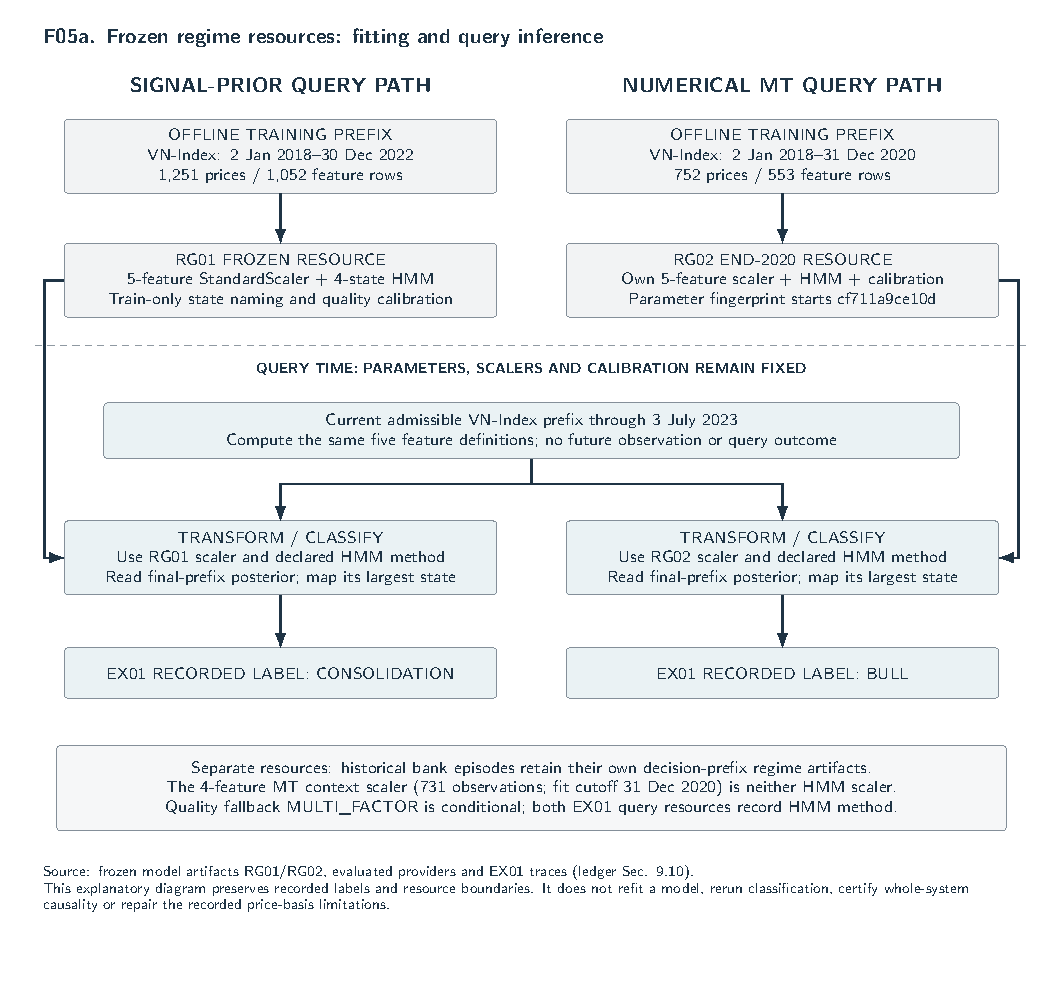
\includegraphics[width=\linewidth,height=0.72\textheight,keepaspectratio]{../assets/diagrams/F05a_regime_training.pdf}
\caption{Separate frozen regime resources and query-time transformations.}\label{fig:F05a}\end{figure}

\emph{Figure F05a. Fitting versus query inference for EX01. Each column retains
its own train-only five-feature HMM scaler, model and calibration. The
current VN-Index prefix can be transformed by either frozen resource without
refitting it. The separate four-feature MT context scaler is not either
HMM scaler. Historical episode-prefix artifacts are a third provenance
path. The diagram describes computation and source identity, not a new fit
or isolated causal effect.} \href{../assets/diagrams/F05a_regime_training.pdf}{PDF}.

\textbf{EX01 identity and assignment.} The signal-prior trace records
CONSOLIDATION from the end-2022 query path; the numeric query records BULL
with feature end date 3 July 2023 and end-2020 model fingerprint beginning
\texttt{cf711a9ce10d}. Both artifacts record HMM method and no quality-fallback
reasons. The model/scaler fingerprints are bound separately in ledger §9.10;
the labels are preserved even though they differ.

The MT context's four-feature scaler is another resource. EX01 records
\texttt{mode=frozen\_\allowbreak{}train}, 731 fitted observations, cutoff 31 December 2020 and
latest fitted exit 29 December 2020. This scaler normalizes context
momentum/volatility/MA-distance observations, not the HMM's five-feature
vector. Its fit-ID hash and full scaler fingerprint distinguish it from the
HMM scalers. Neither model integrity nor a successful regime assignment
resolves the recorded price-basis limitations or certifies overall causal
validity.\footnote{RG01--RG02 frozen model packages, EX01-C and U08 v1 trace; CL062--CL063. The end-2020 fingerprint hashes serialized metadata/model/scaler parameters, while a ZIP-member hash identifies the enclosing artifact bytes. The four-feature context scaler has its own identity; no model or scaler was refitted for this draft.}

\section{Bayesian Prior v1}\label{s:b6cb474a799cc0da}

Bayesian Prior v1 adds a compact description of completed, regime-matched
history to the Common decision request. It asks whether similar agent
conclusions in that market state previously supported a profitable
candidate LONG. Retrieval is categorical and deterministic in this mode;
it is not an embedding search or a new learned trading model. The version's
name also does not mean that its displayed rates are Beta-posterior
probabilities: this implementation reports empirical counts and ratios.
\footnote{BG07 \texttt{prepare\_\allowbreak{}query/\allowbreak{}\_\allowbreak{}select\_\allowbreak{}similarity/\allowbreak{}select\_\allowbreak{}prior\_\allowbreak{}tasks/\allowbreak{}\_\allowbreak{}compute\_\allowbreak{}statistics}, BG16 \texttt{FrozenStudyBank}, SYS20 \texttt{signals}; CL064--CL065 in ledger §9.11. Source describes matching/ranking without economic labels; the mathematical notation is a presentation of that implementation.}

\subsection{Filtering and ranking without outcome-based selection}\label{s:414d3af8992ad0aa}

Let \(E_t\) be the verified same-stock episodes with exit strictly before
cutoff \(t\). The evaluated request fixes \texttt{scope=same\_\allowbreak{}symbol} and
\texttt{mode=bayesian\_\allowbreak{}regime}. Its candidate population is

\[
P_t=\{e\in E_t:\operatorname{regime}(e)=r_t\},
\]

where \(r_t\) is the signal-prior query regime from Section 4.5.4. Bank
identity, exact record contents, date/scope/regime and signal aliases are
validated. A corrupted or out-of-cutoff record is an error, not a candidate
to be silently accepted or repaired.
Checking a stored outcome for economic consistency is an integrity check;
it does not allow its value to determine similarity or ranking.

The query uses the stored Trend, Pattern and Indicator conclusion fields,
the majority direction of Common's five causal Alpha factors, and the
declared sentiment code. The extraction adapter uses the sign of an
available sentiment aggregate, while null/zero becomes its legacy NEUTRAL
code. This differs from live sentiment's \ensuremath{\pm}0.10 labeling and does not convert
missing news into observed evidence. Sentiment must be a valid alias but
does not contribute to v1's similarity score.

For the four scored fields \(F=\{T,P,A,I\}\), normalized to categorical
directions, similarity is

\[
\operatorname{sim}(e,q)=\frac14\sum_{f\in F}\mathbf{1}
\{s_f(e)=s_f(q)\}.
\]

Scores therefore lie in \(\{0,0.25,0.50,0.75,1\}\). Candidates sort by
descending score, then descending exit date, then ascending episode ID.
The selected list has at most \(k\le3\) records; the evaluated setting requests
three. No return, win/loss label or bull-trap outcome enters this ranking.
The seed field is retained in metadata, but this deterministic mode has no
effective random seed. Random/recent/general-similarity controls are
different modes and must not be inferred from this setting.

\subsection{Population statistics and the displayed examples}\label{s:ba7d9ace49327db9}

After eligibility and matching, statistics use \textbf{all of \(P_t\)}, not just
the selected list. LONG win rate counts positive-net candidate cycles over
the full population. Bull-trap rate counts nonpositive-net cycles among
episodes where Trend or Pattern was bullish. Trend-failure and
Pattern-failure rates each use their own bullish subset as denominator.
Trend and Pattern subsets can overlap; their denominators must not be
added as independent evidence. A zero denominator is undefined and appears
as \texttt{0/\allowbreak{}0(N/\allowbreak{}A)}, not an estimated zero risk.

These are unsmoothed descriptive rates; v1 does not compute a credible
interval or fit a Beta posterior here. The LLM may compare this history
with current evidence under the Common instruction. Neither a majority
of winning examples nor a population rate establishes a calibrated query
probability, expected return or compulsory LONG action.

\textbf{EX01 selection.} The pinned bank supplies 211 mature FPT episodes;
19 match CONSOLIDATION. The current scored tuple is bullish Trend,
bullish Pattern, bullish Common Alpha and bearish Indicator. Filtering the
bank first and ranking its 19 matches gives:

\begingroup
\small
\setstretch{1.05}
\setlength{\tabcolsep}{3pt}

\begin{longtable}[]{@{}
  >{\raggedright\arraybackslash}p{(\linewidth - 8\tabcolsep) * \real{0.2000}}
  >{\raggedright\arraybackslash}p{(\linewidth - 8\tabcolsep) * \real{0.2000}}
  >{\raggedright\arraybackslash}p{(\linewidth - 8\tabcolsep) * \real{0.2000}}
  >{\raggedright\arraybackslash}p{(\linewidth - 8\tabcolsep) * \real{0.2000}}
  >{\raggedright\arraybackslash}p{(\linewidth - 8\tabcolsep) * \real{0.2000}}@{}}
\caption{Population statistics and the displayed examples - supporting detail}\label{tab:04_proposed_system:10}\tabularnewline
\toprule\noalign{}
Rank / episode ID
 & T/P/A/I
 & Similarity
 & Exit
 & Saved candidate-LONG result
 \\
\midrule\noalign{}
\endfirsthead
\toprule\noalign{}
Rank / episode ID
 & T/P/A/I
 & Similarity
 & Exit
 & Saved candidate-LONG result
 \\
\midrule\noalign{}
\endhead
\bottomrule\noalign{}
\endlastfoot
1 / \texttt{FPT:\allowbreak{}2022-\allowbreak{}04-\allowbreak{}07} & \texttt{+++-\allowbreak{}} & 1.00 & 13 April 2022 & WIN\_\allowbreak{}IF\_\allowbreak{}LONG, +0.8800636494\% \\
2 / \texttt{FPT:\allowbreak{}2022-\allowbreak{}04-\allowbreak{}18} & \texttt{++0-\allowbreak{}} & 0.75 & 21 April 2022 & LOSS\_\allowbreak{}IF\_\allowbreak{}LONG, \ensuremath{-}4.5332734971\% \\
3 / \texttt{FPT:\allowbreak{}2022-\allowbreak{}04-\allowbreak{}13} & \texttt{++-\allowbreak{}-\allowbreak{}} & 0.75 & 18 April 2022 & LOSS\_\allowbreak{}IF\_\allowbreak{}LONG, \ensuremath{-}0.4389566948\% \\
\end{longtable}

\endgroup

The equal-score pair is ordered by the later exit, not by its return.
The selected list has one win, but the population LONG win rate is
\textbf{9/19}, not 1/3. Its other saved counts are bull trap 9/18, Trend failure
7/14 and Pattern failure 9/18. These are archived-context quantities,
distinct from EX01's later outcome.\footnote{EP01 frozen bank and EX01 U08 v1 retrieval/request; CL066--CL067. Selection/count arithmetic is checked from saved records, with no model call or benchmark replay. The English prefix is labeled as a translation; the original bytes remain archived.}

\subsection{The bounded prefix}\label{s:980a2651ea2ba5dd}

The BRPP renderer emits population/support fields, a legend and the
selected historical lines. The following is an \textbf{English translation for
presentation} of EX01's saved Vietnamese prefix, not the language sent to
the original request:

\begin{Verbatim}[fontsize=\small,breaklines=true,breakanywhere=true]
[BRPP v1] R=CONSOLIDATION; n=19; k=3
LONGwin=9/19(47.4%); Trap=9/18(50.0%); TrendFail=7/14(50.0%); PatternFail=9/18(50.0%)
T/P/A/I: + bullish, - bearish, 0 neutral; W/L=net LONG after costs; SHORT=CASH; S=missing news.
FPT@2022-04-07 R=CONSOLIDATION T/P/A/I=+++- W +0.88%
FPT@2022-04-18 R=CONSOLIDATION T/P/A/I=++0- L -4.53%
FPT@2022-04-13 R=CONSOLIDATION T/P/A/I=++-- L -0.44%
\end{Verbatim}

\texttt{R} identifies the matched regime; \texttt{n} is population size and \texttt{k} the number
of examples. Counts retain their denominators even when percentages are
rounded. T/P/A/I refer to historical conclusions, W/L to the subsequent
candidate LONG after costs, and signed returns use percentage units. The
legend's missing-news notation does not add a fifth scored signal: each
example line displays only T/P/A/I. The v1 formatter accepts this frozen
bank's neutral-coded sentiment, not arbitrary replacement news labels.

The actual saved prefix has \textbf{369 characters}. Insertion plus one newline
changes the EX01 Common prompt from 4,186 to 4,556 characters; removing that
exact substring recovers the archived Common message. The prefix is bounded
at 600 characters and the assembled request must be strictly below 6,500.
Overflow raises an error rather than silently truncating selected examples
or changing support. The renderer checks formatting and count consistency;
the caller must already have verified membership, PIT and provenance.

\subsection{Partial support, bypass and traceability}\label{s:91edd0ea8f0ada5a}

The low-level retriever can return fewer than three examples, with a
\texttt{partial} status, or an empty set with a recorded reason. It does not fill
the list with future, other-regime or undeclared cross-stock episodes.
Its \texttt{k=0} path disables retrieval. Common directly builds an empty-prefix
request and need not load memory merely to represent that control.

A retriever status is distinct from the evaluated wrapper's \textbf{fallback
flag}. For stocks outside the four-stock frozen signal bank, the wrapper
records \texttt{NO\_\allowbreak{}SAME\_\allowbreak{}SYMBOL\_\allowbreak{}FROZEN\_\allowbreak{}BANK\_\allowbreak{}OOD}, empty tasks/null statistics and an
empty prefix. The method adapter verifies equality with the empty-prefix
Common request, then bypasses an additional hosted call. Resolution reuses
the completed \textbf{same-point, same-repeat Common} final action, records
\texttt{FALLBACK\_\allowbreak{}ORIGINAL}, and leaves raw proposal/request/response absent.
Transport, parsing, provenance and cutoff errors still raise; they are not
legitimate evidence-based fallbacks.\footnote{BG16 request wrapper and BG18 \texttt{prepare/\allowbreak{}resolve}, plus FB01 HVN v1/Common U08 slots; CL068--CL069. Dependency hash, missing raw response and bypass are checked separately from the inherited action. F05's source and rendered outputs are bound in ledger §9.11.}

For example, the saved HVN cutoff 3 July 2023, realization 0/repeat 0 trace
has that no-bank reason, null request and null raw v1 response. It points to
the completed Common dependency and retains Common's LONG action. This is
not a second LLM prediction or evidence that the unavailable prior favored
LONG. EX01 FPT itself does not bypass v1. Its population of 19 also does
not trigger the separate minimum-population rule of C2; the following
section distinguishes that readiness logic.

\begin{figure}[htbp]\centering
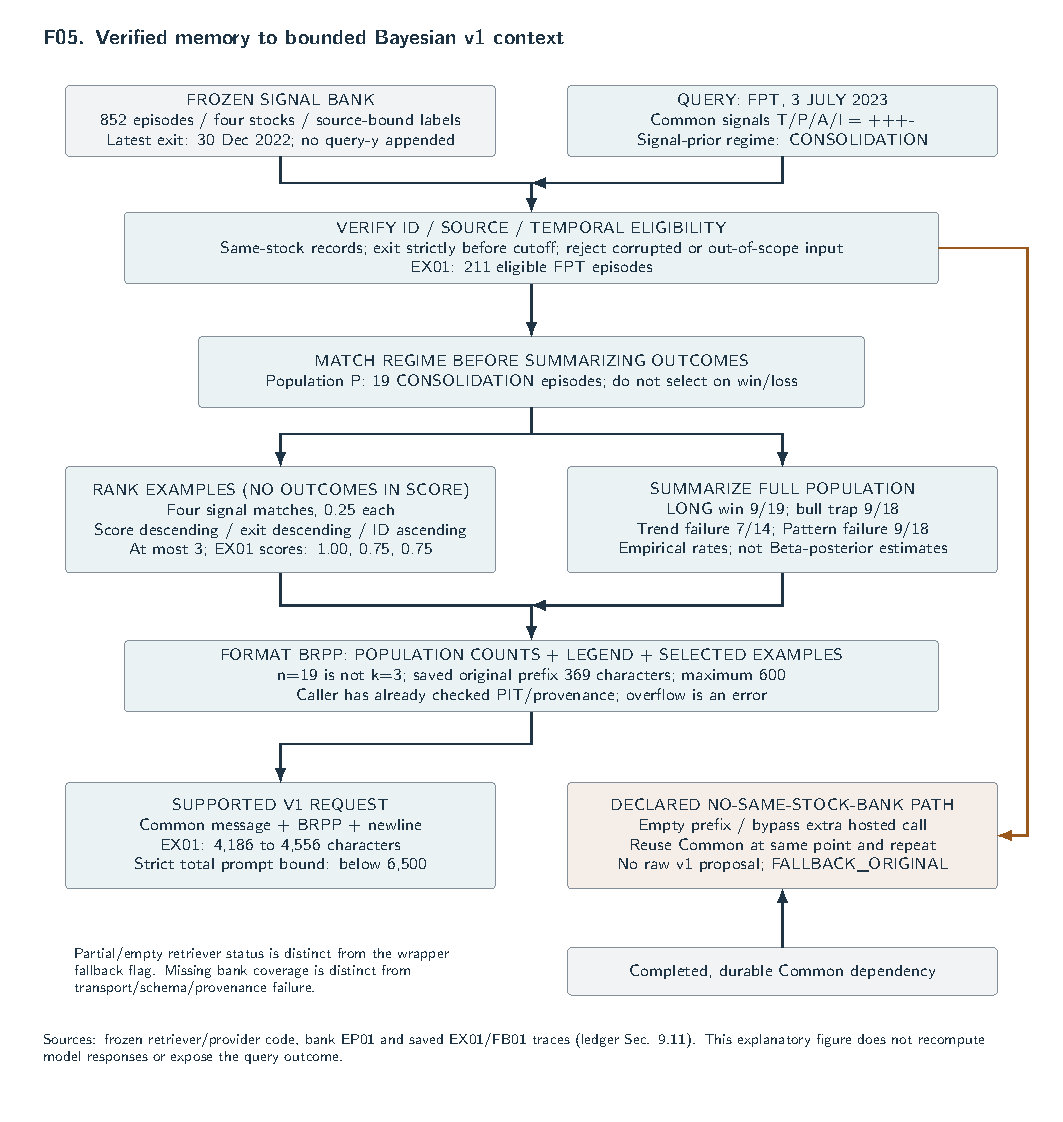
\includegraphics[width=\linewidth,height=0.72\textheight,keepaspectratio]{../assets/diagrams/F05_memory_retrieval.pdf}
\caption{Eligibility, ranking, population statistics and fallback in Bayesian v1.}\label{fig:F05}\end{figure}

\emph{Figure F05. Frozen signal memory to Bayesian v1 context. Membership and
maturity are checked before outcomes are summarized. Population statistics
and at most three ranked examples have separate branches into the prefix.
The declared no-bank path reuses Common from the same point/repeat without
a new hosted response. Counts illustrate the saved FPT EX01 trace; the
diagram does not add a new experiment.} \href{../assets/diagrams/F05_memory_retrieval.pdf}{PDF}.

\section{Conditional and alternative priors}\label{s:280f714ba62ef1fc}

The conditional family separates historical-rate estimation from selecting
examples for the prompt. C2 makes that separation explicit; A and B change
specific parts of its evidence or presentation rather than replacing the
whole pipeline. All retain the temporal/source checks of Section 4.5.

\subsection{C2: disjoint shrinkage and separate readiness}\label{s:928c2fad4a6c3b4b}

\textbf{Population and partition.} Start with the complete verified same-stock,
same-regime population \(\mathcal P\) whose exits precede the cutoff. C2
defines \(\mathcal C\) by exact agreement with the query's four categorical
signals T/P/A/I; sentiment is validated but is not part of this condition.
The disjoint background is \(\mathcal B=\mathcal P\setminus\mathcal C\).
No top-\(k\), age, numerical-feature-availability or example-diversity filter
shrinks these statistical sets. Membership IDs are retained so their
disjointness, completeness and source identity can be checked.
\footnote{BG05 \texttt{compute\_\allowbreak{}conditional\_\allowbreak{}statistics/\allowbreak{}conditional\_\allowbreak{}metric}, with metric masks from BG07; CL070 in ledger §9.12 binds the disjoint groups and plug-in update. Source validation distinguishes outcome consistency from outcome-based retrieval.}

Each metric applies its own event mask inside these same groups. LONG win
counts positive-net candidate cycles over all cycles. Bull-trap support is
the union of bullish Trend or Pattern episodes; success means a
nonpositive-net candidate LONG. Trend/Pattern failure each uses its own
bullish subset. Consequently group cycle counts need not equal a metric's
support counts. For each metric \(h\), both success and support obey
\(s_{p,h}=s_{c,h}+s_{b,h}\) and \(n_{p,h}=n_{c,h}+n_{b,h}\).

\textbf{Shrinkage and interval.} As derived in Section 3.5, C2 forms

\[
\mu_{b,h}=\frac{s_{b,h}+1}{n_{b,h}+2},\quad
a_h=4\mu_{b,h},\quad b_h=4(1-\mu_{b,h}),\quad
\theta_h\mid\mathcal C\sim
\operatorname{Beta}(a_h+s_{c,h},b_h+n_{c,h}-s_{c,h}).
\]

Only conditional counts enter the likelihood; background counts determine
the plug-in prior mean, with strength four. An empty background gives the
fixed symmetric Beta(2,2) prior. An empty \textbf{conditional metric support}
instead leaves posterior shapes, mean and interval absent, with
\texttt{NO\_\allowbreak{}CONDITIONAL\_\allowbreak{}HISTORY}; a prior alone is not displayed as observed
conditional evidence. Nonempty support gives a mean and equal-tailed
2.5\%/97.5\% Beta quantiles. These intervals condition on the estimated
hyperprior and historical event convention. They do not integrate all
hyperparameter uncertainty, establish calibrated query probabilities or
predict net-return magnitudes.

\textbf{Example selection is independent of the statistical partition.} C2
selects from \(\mathcal P\) using four-signal agreement and four-dimensional
price-feature proximity under a source-bound frozen stock/fold scaler.
For standardized vectors \(z_e,z_q\),

\[
d(e,q)=\sqrt{\tfrac14\sum_{j=1}^4(z_{e,j}-z_{q,j})^2},\quad
P(e,q)=\frac1{1+d(e,q)},\quad
B(e,q)=0.5S(e,q)+0.5P(e,q).
\]

Here \(S\) is the v1 four-signal match fraction, while \(B\) denotes a base
similarity, not the background set \(\mathcal B\). Ranking uses
\(B(e,q)2^{-\mathrm{age}/365}\), with age measured from the historical
decision date in calendar days. Candidates need available numerical
features, age at most 730 days and base similarity at least 0.625. Greedy
selection accepts at most three with at least five VN-Index sessions
between decision dates. Ties use later exit, then ascending ID; no random
backfill repairs a short list. Returns do not enter this score. These
selection restrictions do not delete cycles from the rate population.
\footnote{SYS26/SYS27 example selection and signal/price scoring, BG06 split quality gate; CL071--CL072. The evaluated settings are confirmed in EX01's saved selection metadata; no index or scaler is refitted here.}

\textbf{Readiness is evaluated before projection.} A metric can be visible when
population size is at least 20, that metric's conditional support is at
least five, and its 95\% interval width is at most 0.75. Equality passes
each bound; calculations use unrounded values. \texttt{stats\_\allowbreak{}ready} means at
least one metric passes, not that all four pass. Examples require the same
population floor, available query features and scaler, and a nonempty
selected list. They do not require five exact T/P/A/I matches or a narrow
rate interval. Thus either block can be ready while the other is unavailable.

The full-prior view exposes whichever blocks pass. Stats-only and
examples-only views can fallback independently when their requested block
is absent. No visible block means an empty prefix and reuse of the
same-repeat Common result; missing/corrupt artifacts are technical errors,
not low-evidence fallbacks. Disabling the prior or setting \(k=0\) skips
statistical/index selection work under an explicit disabled state.

\textbf{EX01 counts and withheld content.} Its population has 19 episodes.
Only \texttt{FPT:\allowbreak{}2022-\allowbreak{}04-\allowbreak{}07} matches the query's T/P/A/I tuple, so \(|\mathcal C|=1\)
and \(|\mathcal B|=18\). The saved evidence contains:

\begingroup
\small
\setstretch{1.05}
\setlength{\tabcolsep}{3pt}

\begin{longtable}[]{@{}
  >{\raggedright\arraybackslash}p{(\linewidth - 10\tabcolsep) * \real{0.1667}}
  >{\raggedright\arraybackslash}p{(\linewidth - 10\tabcolsep) * \real{0.1667}}
  >{\raggedright\arraybackslash}p{(\linewidth - 10\tabcolsep) * \real{0.1667}}
  >{\raggedright\arraybackslash}p{(\linewidth - 10\tabcolsep) * \real{0.1667}}
  >{\raggedright\arraybackslash}p{(\linewidth - 10\tabcolsep) * \real{0.1667}}
  >{\raggedright\arraybackslash}p{(\linewidth - 10\tabcolsep) * \real{0.1665}}@{}}
\caption{C2: disjoint shrinkage and separate readiness - supporting detail}\label{tab:04_proposed_system:11}\tabularnewline
\toprule\noalign{}
Metric
 & Population success/support
 & Conditional success/support
 & Background success/support
 & Posterior mean
 & 95\% interval
 \\
\midrule\noalign{}
\endfirsthead
\toprule\noalign{}
Metric
 & Population success/support
 & Conditional success/support
 & Background success/support
 & Posterior mean
 & 95\% interval
 \\
\midrule\noalign{}
\endhead
\bottomrule\noalign{}
\endlastfoot
LONG win & 9/19 & 1/1 & 8/18 & 0.560000 & {[}0.163553, 0.912248{]} \\
Bull trap & 9/18 & 0/1 & 9/17 & 0.421053 & {[}0.077883, 0.822315{]} \\
Trend failure & 7/14 & 0/1 & 7/13 & 0.426667 & {[}0.080748, 0.826566{]} \\
Pattern failure & 9/18 & 0/1 & 9/17 & 0.421053 & {[}0.077883, 0.822315{]} \\
\end{longtable}

\endgroup

For LONG win, \((8+1)/(18+2)=0.45\) yields prior shapes (1.8,2.2)
and posterior (2.8,2.2). These stored estimates are auditable even though
they are not ready for the prompt. All four widths are below 0.75, but
population 19 is below 20 and every conditional support is one, below five.
The numerical selector separately finds three records: 7 April,
25 March and 4 March 2022. They are not the v1 displayed list, and they
are not all in \(\mathcal C\).

C2's \texttt{retrieved\_\allowbreak{}k=3} therefore coexists with \texttt{effective\_\allowbreak{}k=0}, no ready
metric IDs, no visible examples, an empty prefix and no additional hosted
C2 response. EX01 retains Common's LONG via \texttt{FALLBACK\_\allowbreak{}ORIGINAL}. It would
be incorrect to describe the posterior table above as content actually
seen by that Decision request.\footnote{U08 EX01 C2 prepared trace, raw groups/metrics, selection, request and policy; CL073. Counts and Beta arithmetic are checked against saved evidence; this is not a new forecast or a rerun of the statistical pipeline.}

\subsection{Alternative conditional and presentation profiles}\label{s:ae882769bc20ece1}

\textbf{A: pool the conditional statistics by Trend/Pattern.} \texttt{A\_\allowbreak{}tp\_\allowbreak{}pool} keeps
the same same-stock/same-regime population \(\mathcal P\), but defines
\(\mathcal C_A\) by exact T/P agreement alone. Alpha and Indicator no longer
split the statistical condition; the disjoint background remains
\(\mathcal P\setminus\mathcal C_A\). The metric masks, strength-four plug-in
update and split readiness thresholds remain those of C2. ``Pool'' here
does not mean pooling other stocks, regimes or future observations.
\footnote{SYS25 \texttt{tp\_\allowbreak{}statistics/\allowbreak{}build\_\allowbreak{}evidence/\allowbreak{}render\_\allowbreak{}prefix/\allowbreak{}PROFILES}, SYS28 C2 renderer, BG06 split views and SYS26/SYS27 selector; CL074--CL075 and ledger §9.13. The table describes evaluated base profiles and separates their registered content modes.}

The example selector is unchanged: it still uses T/P/A/I plus numerical
price similarity, recency and session diversity. Loosening the statistical
condition does not loosen its four-signal score or replace examples with
all T/P matches. A recomputes its conditional statistics, gate and visible
content views, then marks the compact prefix as a T/P profile. The base
evidence hash therefore changes when statistical membership changes.

\textbf{B: change presentation while retaining C2 evidence.} \texttt{B\_\allowbreak{}semantic} reuses
C2's statistical partition, posterior, example selection and readiness.
It changes the bounded renderer: short event labels W/BT/TF/PF are paired
with definitions, conditional success/support counts, posterior mean and
95\% interval, and an explicit warning that the values are historical rates,
not query probability or expected return. Historical example lines retain
their IDs and outcomes. C2's renderer already includes counts and intervals;
B reorganizes their wording and notation rather than introducing those
quantities for the first time.

The name ``semantic'' refers to this presentation profile. There is no
embedding encoder, vector search over report meaning or language-model
retrieval step in this implementation. C2 and B have the same base-evidence
hash for the same query/settings. Their rendered prefix/request identities
can differ when content is visible. In a bypassed case both prefixes can
be empty, so the archived trace must be checked before claiming that a
presentation contrast actually reached the model.

\emph{Table B03, prior-family portion. Together with the foundation portion in
Section 4.4, this identifies the four historical-prior interventions. All
use verified mature same-stock evidence and the Common decision foundation;
the final orchestration/dependency table appears in Section 4.9.}

\begingroup
\small
\setstretch{1.05}
\setlength{\tabcolsep}{3pt}

\begin{longtable}[]{@{}
  >{\raggedright\arraybackslash}p{(\linewidth - 8\tabcolsep) * \real{0.2000}}
  >{\raggedright\arraybackslash}p{(\linewidth - 8\tabcolsep) * \real{0.2000}}
  >{\raggedright\arraybackslash}p{(\linewidth - 8\tabcolsep) * \real{0.2000}}
  >{\raggedright\arraybackslash}p{(\linewidth - 8\tabcolsep) * \real{0.2000}}
  >{\raggedright\arraybackslash}p{(\linewidth - 8\tabcolsep) * \real{0.2000}}@{}}
\caption{Table B03, prior-family portion. Together with the foundation portion in Section 4.}\label{tab:04_proposed_system:12}\tabularnewline
\toprule\noalign{}
Family
 & Statistical population and conditioning
 & Examples
 & Visible representation
 & Support and dependency
 \\
\midrule\noalign{}
\endfirsthead
\toprule\noalign{}
Family
 & Statistical population and conditioning
 & Examples
 & Visible representation
 & Support and dependency
 \\
\midrule\noalign{}
\endhead
\bottomrule\noalign{}
\endlastfoot
v1 (\texttt{bayesian\_\allowbreak{}v1}) & Same regime; unsmoothed population ratios, no exact-signal conditional posterior & Four-signal score; exit/ID tie-break, at most three & \texttt{compact\_\allowbreak{}brpp\_\allowbreak{}v1}: population counts, legend and historical lines & Retriever can be partial/empty; declared no-bank wrapper bypass reuses same-repeat Common. C2 floors do not apply. \\
C2 & Same regime; exact T/P/A/I conditional set and disjoint background; plug-in Beta summaries & Signal/price similarity, recency, age/similarity bounds and five-session diversity & \texttt{compact\_\allowbreak{}brpp\_\allowbreak{}v3}: ready conditional counts, mean/interval and/or ready examples & Split metric/example gate; no visible block or no same-stock bank reuses same-repeat Common \\
A (\texttt{A\_\allowbreak{}tp\_\allowbreak{}pool}) & Same regime; exact T/P conditional set and disjoint background; same shrinkage recipe & Identical four-signal/price selector to C2 & \texttt{compact\_\allowbreak{}brpp\_\allowbreak{}v3\_\allowbreak{}tp\_\allowbreak{}v1}: C2-style content labeled as T/P conditioning & Recompute split gate after changing statistics; Common dependency when no visible block \\
B (\texttt{B\_\allowbreak{}semantic}) & Identical to C2, including its base evidence & Identical to C2 & \texttt{compact\_\allowbreak{}brpp\_\allowbreak{}semantic\_\allowbreak{}v1}: short event names with explicit meanings/counts and plug-in disclaimer & Identical readiness to C2; changed wording can reach Decision only when a block is visible \\
\end{longtable}

\endgroup

The base profiles in this study request \texttt{full\_\allowbreak{}prior}: ready statistics
and/or examples. Registered stats-only and examples-only content modes
project the same base evidence; they do not select a new statistical
population. Their availability and actual execution belong to the protocol
of the panel using them. Every prefix remains bounded at 600 characters,
with overflow treated as an error rather than dropping evidence.

\textbf{EX01 comparison.} A enlarges the conditional set from one to 14 cycles,
leaving five background cycles. Its saved counts are:

\begingroup
\small
\setstretch{1.05}
\setlength{\tabcolsep}{3pt}

\begin{longtable}[]{@{}
  >{\raggedright\arraybackslash}p{(\linewidth - 6\tabcolsep) * \real{0.1800}}
  >{\raggedright\arraybackslash}p{(\linewidth - 6\tabcolsep) * \real{0.2700}}
  >{\raggedright\arraybackslash}p{(\linewidth - 6\tabcolsep) * \real{0.2800}}
  >{\raggedright\arraybackslash}p{(\linewidth - 6\tabcolsep) * \real{0.2700}}@{}}
\caption{Alternative conditional and presentation profiles - supporting detail}\label{tab:04_proposed_system:13}\tabularnewline
\toprule\noalign{}
Metric
 & A conditional success/support
 & A background success/support
 & A posterior mean
 \\
\midrule\noalign{}
\endfirsthead
\toprule\noalign{}
Metric
 & A conditional success/support
 & A background success/support
 & A posterior mean
 \\
\midrule\noalign{}
\endhead
\bottomrule\noalign{}
\endlastfoot
LONG win & 7/14 & 2/5 & 0.484127 \\
Bull trap & 7/14 & 2/4 & 0.500000 \\
Trend failure & 7/14 & 0/0 & 0.500000 \\
Pattern failure & 7/14 & 2/4 & 0.500000 \\
\end{longtable}

\endgroup

The Trend background denominator is zero even though the background group
has five cycles: none had bullish Trend. Its symmetric prior is therefore
metric-specific. The population counts still equal the C2 population
counts. Selected example IDs also remain 7 April, 25 March and 4 March
2022. C2 and B retain the same 1/18 conditional/background split and the
same base-evidence fingerprint. A has a different fingerprint.

All three nevertheless fail EX01's population floor, since 19 is below
20. Their visible prefixes are empty, their own raw responses are absent
and their final actions inherit the same-repeat Common LONG. The example
demonstrates different evidence construction with a shared bypass, not an
observed LLM response to A's broader statistics or B's alternative wording.
\footnote{EX01 C2/A/B prepared evidence/request and dependency/policy records in U08, joined to EP01 bank; CL076--CL077. Exact C2/B evidence equality, A counts and empty visible content are verified without rendering a new research request or invoking an LLM.}

\section{MT-BICL and action revision}\label{s:2d298f46dad25b7a}

MT-BICL adds a numerical context built from mature historical observations,
not a collection of new LLM agents trained on query outcomes. Task selection,
frozen numerical teacher/student inference, hosted language-model proposals
and external action resolution are separate operations. The following
subsections explain their inputs and boundaries before describing utility
and the complete revision policy. An available numerical context alone does
not authorize an action change.

\subsection{Fact packet and Fact Anchor}\label{s:20f38305181c1972}

Fact Anchor establishes the reference action \(a_0\) for the later revision
stage. It combines source-bound numerical facts with the Common-profile
reports, then checks a small structured assertion contract in the returned
reply. It has a declared dependency on Common from the same point and
repeat. It does not compute a return threshold or apply a utility veto.
\footnote{BG10 fact-packet construction, SYS33 fact/wire validator, SYS42 fact-card/anchored builder and BG18 Common dependency. CL089--CL090 and ledger §9.16 distinguish raw prefix provenance, numerical consistency and reply schema.}

\textbf{Facts from the admissible price prefix.} \texttt{make\_\allowbreak{}fact\_\allowbreak{}packet} takes the
last 45 observed OHLCV bars ending at the query cutoff. It obtains MACD
(12,26,9) from TA-Lib and the last-20-close mean, retaining full-precision
numbers and their differences. It emits three assertion IDs:

\begingroup
\small
\setstretch{1.05}
\setlength{\tabcolsep}{3pt}

\begin{longtable}[]{@{}
  >{\raggedright\arraybackslash}p{(\linewidth - 4\tabcolsep) * \real{0.2400}}
  >{\raggedright\arraybackslash}p{(\linewidth - 4\tabcolsep) * \real{0.3900}}
  >{\raggedright\arraybackslash}p{(\linewidth - 4\tabcolsep) * \real{0.3700}}@{}}
\caption{Fact packet and Fact Anchor - supporting detail}\label{tab:04_proposed_system:14}\tabularnewline
\toprule\noalign{}
Assertion ID
 & Relationship checked
 & Admitted values
 \\
\midrule\noalign{}
\endfirsthead
\toprule\noalign{}
Assertion ID
 & Relationship checked
 & Admitted values
 \\
\midrule\noalign{}
\endhead
\bottomrule\noalign{}
\endlastfoot
\texttt{MACD\_\allowbreak{}SIGNAL} & MACD line relative to its Signal & ABOVE, BELOW, EQUAL or UNKNOWN \\
\texttt{MACD\_\allowbreak{}ZERO} & MACD line relative to zero & POSITIVE, NEGATIVE, ZERO or UNKNOWN \\
\texttt{PRICE\_\allowbreak{}SMA20} & Last Close relative to SMA20 & ABOVE, BELOW, EQUAL or UNKNOWN \\
\end{longtable}

\endgroup

These are distinct relationships: being below Signal does not mean MACD
is below zero. Comparisons use stored unrounded numbers, and exact equality
is distinct from unavailable data. The packet also carries point/cutoff,
frame end, prefix length, horizon, bucket and a hash of the actual input
prefix. Fewer than 45 bars or a window ending before cutoff does not permit
finite numerical facts to be asserted as if the complete window existed.
Invalid OHLCV or inconsistent fields are errors.

The packet validator checks schema, dates, raw numerical differences and
the assertion/bucket relations. The source adapter must still establish
the price prefix's identity; a self-consistent packet or self-recomputed
hash is not independent evidence that its source is authentic. Optional
report warnings are labeled as report statements, not promoted to hard
numerical assertions.

Matching UNKNOWN likewise does not supply a missing observation or satisfy
the later context-support gate.

\textbf{Prompt and structured reply.} The Fact Anchor request includes the fact
card and the same Common-projected reports. It does not include an MT task
projection, student probability or utility distribution. The instruction
asks the model to cite all three IDs/assertions and use
\texttt{context\_\allowbreak{}reason=NOT\_\allowbreak{}APPLICABLE}. Fact-card numbers are displayed with eight
significant digits, while validation retains the original values and enums.
The fact card has its own 700-character bound; the final assembled request
remains strictly below 6,500 characters. It is not a 600-character BRPP.
The branch also changes instructions and the output schema; a comparison
with Common therefore combines fact presentation and response-format changes.

The reply schema retains decision, horizon, confidence, R:R and explanatory
fields, and adds a version, the three unique \texttt{fact\_\allowbreak{}ids}, a
\texttt{fact\_\allowbreak{}assertions} object and \texttt{context\_\allowbreak{}reason}. Citation completeness is
checked as a set, so changing ID order alone does not invalidate the reply.
Schema validity only establishes allowed fields and values; it does not
prove that the returned values agree with the packet.

\textbf{Resolve the anchor before any action revision.} The policy compares the
reply's assertion object exactly with the packet and requires the
Fact Anchor context reason to be NOT\_\allowbreak{}APPLICABLE. If both checks pass,
\(a_0\) is the reply's decision mapped to LONG/CASH. A valid SHORT reply
therefore yields CASH under the economic contract. If a schema-valid reply
has incorrect assertions or context reason, the resolver instead uses
the already completed Common reply and records
\texttt{ANCHOR\_\allowbreak{}INVALID\_\allowbreak{}USE\_\allowbreak{}ORIGINAL}. This fallback does not certify the Common
reply's prose or supply it with new fact assertions.

The proof retains the packet hash, Common source/output hash, anchor source
hash, raw replies, validity flag and request ID. The selected reference
action can be reconstructed from those fields. An invalid completed anchor
still has a real request/raw reply and \texttt{bypass=False} for that anchor call.
Its validity flag remains false; a later anchored revision is bypassed
rather than sending a new revision request based on an invalid anchor.
A missing response, malformed schema, corrupt provenance or transport
failure is a technical failure, not a completed invalid assertion reply
that can silently be replaced with CASH.\footnote{BG14 \texttt{facts\_\allowbreak{}match/\allowbreak{}resolve\_\allowbreak{}anchor/\allowbreak{}validate\_\allowbreak{}anchor/\allowbreak{}apply\_\allowbreak{}revision} and BG18 \texttt{prepare/\allowbreak{}resolve}; CL091. The invalid example is explicitly illustrative and does not add a new research response or replace a transport failure.}

\textbf{EX01 numerical assertions.} The saved packet records:

\begingroup
\small
\setstretch{1.05}
\setlength{\tabcolsep}{3pt}

\begin{longtable}[]{@{}
  >{\raggedright\arraybackslash}p{(\linewidth - 2\tabcolsep) * \real{0.3000}}
  >{\raggedright\arraybackslash}p{(\linewidth - 2\tabcolsep) * \real{0.7000}}@{}}
\caption{Fact packet and Fact Anchor - supporting detail}\label{tab:04_proposed_system:15}\tabularnewline
\toprule\noalign{}
Quantity / assertion
 & Stored value
 \\
\midrule\noalign{}
\endfirsthead
\toprule\noalign{}
Quantity / assertion
 & Stored value
 \\
\midrule\noalign{}
\endhead
\bottomrule\noalign{}
\endlastfoot
MACD / Signal & 0.6542675609756259 / 0.7043937016476567 \\
MACD \ensuremath{-} Signal & \ensuremath{-}0.050126140672030806; \texttt{MACD\_\allowbreak{}SIGNAL=BELOW} \\
MACD relative to zero & \texttt{MACD\_\allowbreak{}ZERO=POSITIVE} \\
Close / SMA20 & 48.18 / 47.5675 \\
Close \ensuremath{-} SMA20 & 0.6124999999999972; \texttt{PRICE\_\allowbreak{}SMA20=ABOVE} \\
Facts bucket & \texttt{MACD\_\allowbreak{}NEG\_\allowbreak{}PRICE\_\allowbreak{}POS} \\
\end{longtable}

\endgroup

The anchor reply cites all three matching assertions with
NOT\_\allowbreak{}APPLICABLE, proposes LONG, states high confidence and R:R 1.5. Its
reference/final action is LONG with \texttt{NO\_\allowbreak{}NUMERIC\_\allowbreak{}VETO}; the utility-quantile
field is null. Common's separate reply also proposes LONG, but with R:R
2.5. The anchor request has 3,916 characters and its source request ID
begins \texttt{f7c7664b-\allowbreak{}69c7}; the ledger binds the full ID and source hashes.

This valid structured reply nevertheless illustrates the check's limit.
Its prose calls MACD below Signal bullish momentum and refers to a positive
zero crossing. The equality of the three returned enums does not validate
that interpretation, and an endpoint-positive MACD does not by itself
establish a crossing event. \texttt{fact\_\allowbreak{}assertions\_\allowbreak{}valid=True} must therefore be
read as the limited citation/enum contract, not a certificate that all prose,
trading logic or future profit is correct.\footnote{EX01 U08 Fact\_\allowbreak{}Anchor prepared packet/request, raw reply and policy/proof, linked to Common r0; CL092. Exact assertions, source identity, prompt length and the saved prose limitation are checked without rerunning TA-Lib or a model.}

\textbf{Illustrative invalid-anchor branch, not an archived response.} Suppose
a schema-valid reply on the EX01 packet proposes SHORT but returns
\texttt{MACD\_\allowbreak{}ZERO=NEGATIVE}. The packet's positive MACD makes the assertion
comparison fail. The resolver records the raw SHORT proposal while taking
\(a_0=\mathrm{LONG}\) from the saved Common reply, with validity false and
ANCHOR\_\allowbreak{}INVALID\_\allowbreak{}USE\_\allowbreak{}ORIGINAL. The later revision path retains that reference
without a new revision call. No return estimate or quantile comparison is
needed to explain this branch; utility-based acceptance or rejection belongs
to Section 4.8.6.

\subsection{Task construction}\label{s:673616bb765d15ae}

\textbf{An observation and its four-dimensional input.} A numerical observation
is one completed candidate LONG cycle. Its feature vector is computed at
the historical decision from a valid 21-session price segment:

\[
x_i=\left(
\frac{C_i}{C_{i-5}}-1,\quad
\frac{C_i}{C_{i-20}}-1,\quad
\operatorname{Std}_{\mathrm{pop}}\{\log(C_u/C_{u-1})\}_{u=i-19}^{i},\quad
\frac{C_i}{\operatorname{SMA}_{20}(C)_i}-1
\right).
\]

The volatility uses population standard deviation (\texttt{ddof=0}), distinct
from the HMM's sample-volatility feature. Missing sessions, invalid prices
or a relevant corporate-action barrier can make the segment unavailable;
the pipeline does not fill a missing session with a synthetic candle.
The cycle's historical label is \(y_i=\mathbf1\{r_i^{\mathrm{net}}>0\}\),
using the canonical execution oracle and costs. The saved \texttt{r\_\allowbreak{}net} is a
sidecar for historical utility/evidence, not an extra coordinate in \(x_i\).
\footnote{SYS29 PIT feature primitive, BG08 numerical bank, SYS31 scaler and SYS32 stream, with BG23's frozen-resource adapter; CL078--CL079 in ledger §9.14. Pinned source and artifact determine the evaluated feature and scaling conventions.}

The four-feature scaler uses admitted closed training observations, with
population variance per coordinate. Zero-variance coordinates use scale
one. The model receives \(v_i=\operatorname{clip}((x_i-\mu)/\sigma,-4,4)\);
raw \(x_i\) and unclipped standardized \(z_i\) remain in the record. Early
training-prefix construction respects its own strict exit cutoff; after
2020 the evaluated path reuses the frozen end-2020 scaler, not a scaler
refitted on each query's 600 bars. This is also distinct from the
stock/fold scaler of C2 example retrieval and from either HMM scaler.

\textbf{A task is a stock/block group.} VN-Index's observed-session calendar is
anchored on 2 January 2018. For zero-based calendar index \(i\), block
\(b=\lfloor i/63\rfloor\) defines task \texttt{symbol:\allowbreak{}blockNNNN}. Candidate cycles
follow a three-session grid and must stay within their admitted block and
partition. A prior task comes from an earlier block of the \textbf{same stock};
target observations come from the query's own block. This grouping permits
within-task context while retaining differences across historical blocks.
It does not assert that a market process resets every 63 sessions.

\textbf{Filter by a numerical facts bucket before task selection.} The evaluated
\texttt{BucketTaskBuilder} first restricts mature available candidates to the
query's factual bucket. Its axes are the signs of MACD minus Signal and
Close minus SMA20, computed on each decision's own 45-bar prefix with the
same definitions as the query. Strict positive/negative comparisons are
made before rounding. A zero or missing axis gives UNKNOWN; that query
has no selected bucket context. These are price-derived buckets, not the
directions asserted in a generated report, and they are distinct from the
VN-Index HMM regime.\footnote{BG09 task builder, BG10 bucket/facts view, SYS33 membership validator and BG16/BG17 freeze/reserved adapters; CL080--CL081. Matching uses admissible numerical facts before selection, while metadata validation is separate from scientific certification.}

For each earlier block with at least two admitted observations, the builder
computes a centroid using \textbf{all} its eligible clipped model vectors. Tasks
rank first by a known regime match to the query, then by smaller Euclidean
centroid distance, later latest exit and task ID. Regime agreement is a
priority, not an absolute filter that forbids every unmatched task.
At most three prior tasks are kept. Within each, at most eight observations
are chosen by distance to the query, with more recent decision date and
ID breaking ties, then presented chronologically. Target context instead
keeps the latest at most eight eligible observations in the current block;
it is not selected by the prior-task nearest-neighbor rule.

Every selected historical exit must strictly precede the query, and
observation IDs and holding intervals must remain disjoint. In the context
study, the labeled stream is additionally frozen before the first query
of each fold and withholds the reserved evaluation IDs, as described in
Section 4.5.2. Query features and bucket can change at later cutoffs, but
that does not admit new within-fold labels. Data shortage has explicit
reasons such as a cold target or fewer prior tasks; no winning examples
are inserted to improve a selected context.

The context preserves full membership, selected-by-distance IDs,
centroid-fit IDs, scaler, raw facts and regime proofs. Its membership hash
binds query/scaler/prior/target/advisor objects, not only a short displayed
ID list. Facts for the centroid population are retained even when some
population observations are not among the eight encoded examples.
The network input projection preserves task boundaries and labeled
historical pairs, while keeping the query unlabeled; its packing is
explained next.

\textbf{EX01 numerical context.} The query's calendar index is 1,372, giving
block 21 and task \texttt{FPT:\allowbreak{}block0021}. Its bucket is
\texttt{MACD\_\allowbreak{}NEG\_\allowbreak{}PRICE\_\allowbreak{}POS}. This means MACD is below its Signal while Close is
above SMA20; it does not mean that MACD itself is negative. Its raw vector
is approximately (0.007107, 0.016456, 0.007498, 0.012876), and the model
vector is (0.109634, 0.101272, \ensuremath{-}1.290443, 0.215713). No coordinate is clipped
in this case. The scaler has 731 fitted observations and the identity
already recorded in Section 4.5.4.

\begingroup
\small
\setstretch{1.05}
\setlength{\tabcolsep}{3pt}

\begin{longtable}[]{@{}
  >{\raggedright\arraybackslash}p{(\linewidth - 6\tabcolsep) * \real{0.1800}}
  >{\raggedright\arraybackslash}p{(\linewidth - 6\tabcolsep) * \real{0.2700}}
  >{\raggedright\arraybackslash}p{(\linewidth - 6\tabcolsep) * \real{0.2800}}
  >{\raggedright\arraybackslash}p{(\linewidth - 6\tabcolsep) * \real{0.2700}}@{}}
\caption{Task construction - supporting detail}\label{tab:04_proposed_system:16}\tabularnewline
\toprule\noalign{}
Context group
 & Task
 & Selected observations
 & Latest selected exit
 \\
\midrule\noalign{}
\endfirsthead
\toprule\noalign{}
Context group
 & Task
 & Selected observations
 & Latest selected exit
 \\
\midrule\noalign{}
\endhead
\bottomrule\noalign{}
\endlastfoot
Prior P1 & \texttt{FPT:\allowbreak{}block0011} & 5 & 29 December 2020 \\
Prior P2 & \texttt{FPT:\allowbreak{}block0015} & 4 & 29 November 2021 \\
Prior P3 & \texttt{FPT:\allowbreak{}block0013} & 2 & 14 July 2021 \\
Target T & \texttt{FPT:\allowbreak{}block0021} & 3 & 29 June 2023 \\
Query Q & \texttt{FPT:\allowbreak{}block0021} & One unlabeled feature vector & No observed outcome in context \\
\end{longtable}

\endgroup

Thirty eligible bucket-filtered observations precede selection. The selected
context has \(K=3\) prior tasks containing 11 observations, plus \(m=3\) target
observations: 14 labeled rows, not three rows. The target decision dates
are 16, 21 and 26 June 2023, with exits on 21, 26 and 29 June. Calendar
entry/exit dates attached to Q specify the horizon; they do not expose its
future execution prices or label. The saved context's membership hash
begins \texttt{9ed7e2a35da5} and is linked to the hosted MT preparation.
\footnote{EX01-C and the U08 MT preparation, source identity in §7 and scaler identity in §9.10; CL082. The illustrative F06 layout uses those saved counts and no query outcome.}

\begin{figure}[htbp]\centering
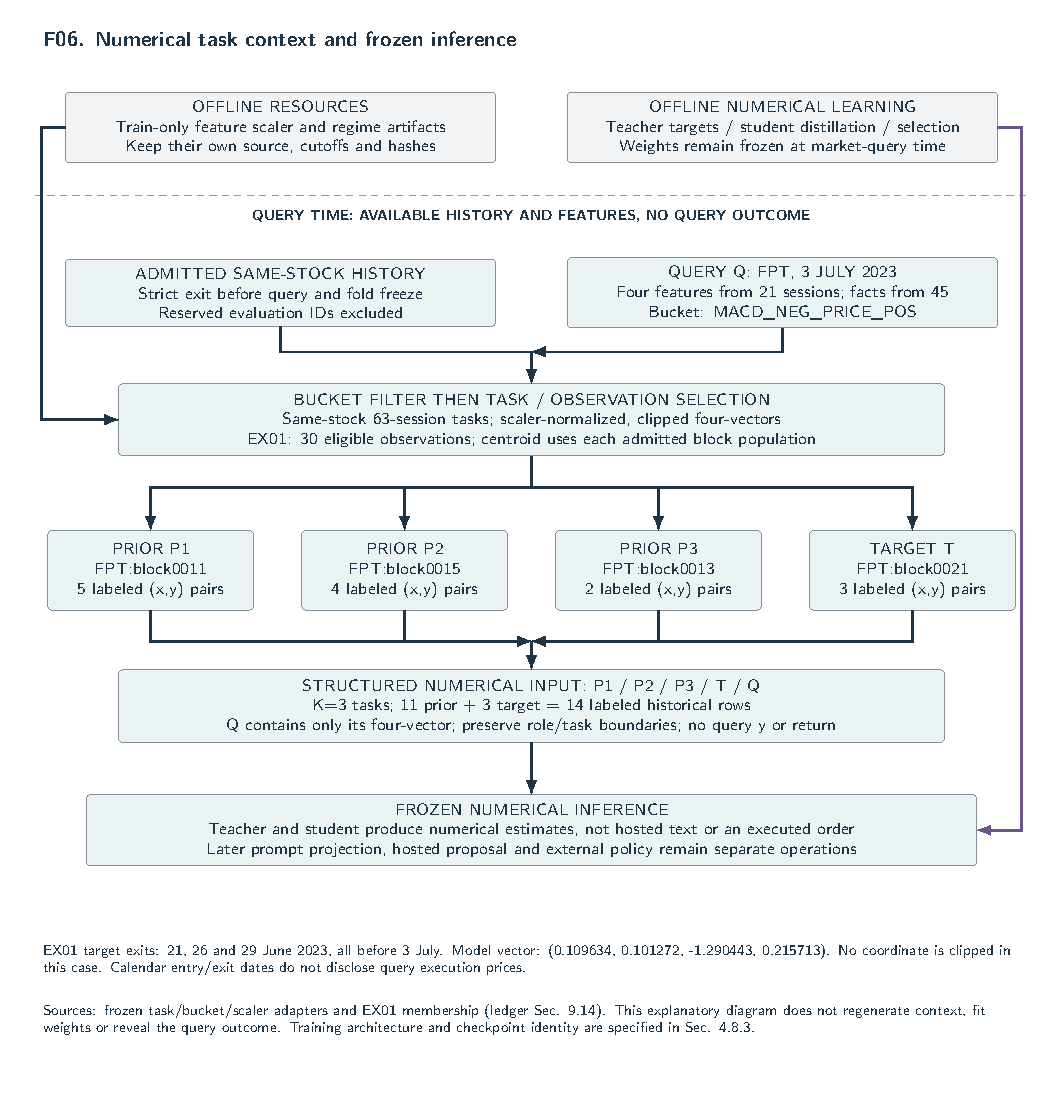
\includegraphics[width=\linewidth,height=0.72\textheight,keepaspectratio]{../assets/diagrams/F06_mt_tasks_training.pdf}
\caption{Task membership, masked query and frozen numerical inference.}\label{fig:F06}\end{figure}

\emph{Figure F06. Numerical context and the offline/query boundary. P1--P3 and T
contain distinct mature labeled observations; Q supplies only its feature
vector. Task selection and numerical inference use frozen resources, while
the later hosted decision and action policy are separate. EX01 counts come
from the saved membership, not a regenerated model run. Teacher/student
training details follow in Section 4.8.3.}
\href{../assets/diagrams/F06_mt_tasks_training.pdf}{PDF}.

\subsection{Teacher and student}\label{s:54ebb2a16a274585}

This stage trains a small numerical student offline to approximate a
registered Bayesian teacher on structured task contexts. The evaluated
resource is \texttt{MT\_\allowbreak{}BICL\_\allowbreak{}replica\_\allowbreak{}full\_\allowbreak{}r1}. The hosted Decision LLM consumes a
later text projection; it is not the student whose weights are trained
here. The theoretical motivation in Section 3.6 does not substitute for
this implementation's architecture, training distribution or selected
checkpoint.\footnote{Frozen model-asset manifest TR01 and recipe TR02 identify the evaluated replica, rather than module defaults or the earlier model release. BG23/BG16/BG17 bind reuse in the context study. CL083--CL088 and ledger §9.15 distinguish recorded resource acceptance from whole-system certification.}

\textbf{Teacher fit.} The teacher has 16 fixed Beta components, formed by
\(\mu\in\{0.2,0.4,0.6,0.8\}\) and
\(\kappa\in\{2,8,32,128\}\), with \(a_h=\mu_h\kappa_h\) and
\(b_h=(1-\mu_h)\kappa_h\). Only mixture weights \(\pi_h\) are fitted. The
saved fit uses 731 available training cycles in 48 unique stock/block tasks,
with exits through end-2020. Each task contributes its label counts once;
reusing the same task at several queries does not duplicate its fitting
weight. Labels are checked against the canonical net-return oracle.

For task counts \((s,f)\) the likelihood is
\(L_h(s,f)=B(a_h+s,b_h+f)/B(a_h,b_h)\). MAP-EM starts with uniform weights,
uses a symmetric \(\operatorname{Dirichlet}(2,\ldots,2)\) prior, and updates
\(\pi_h=(\sum_j\gamma_{jh}+1)/(N_{\mathrm{tasks}}+16)\).
The grid is fixed; there is no search for new component shapes on query
data. The registered limit is 1,000 iterations with maximum weight change
below \(10^{-10}\) required for convergence. The saved teacher converged in
237 iterations. Nonconvergence would stop preparation, not substitute a
uniform teacher.\footnote{BG11 teacher likelihood/fit/predict and TR03 saved teacher; 48 tasks/731 cycles/237 iterations are artifact values. The Bayesian derivation in Section 3.6 describes this convention; it does not claim generic equivalence to an external architecture.}

\textbf{Conditioning at inference.} A latent family is shared across prior and
target tasks in the teacher's episode model, with separate task-specific
Bernoulli rates given that family. For visible prior-task counts
\((s_j,f_j)\) and target counts \((s_T,f_T)\),

\[
w_h\propto\pi_h\left[\prod_{j=1}^{K}L_h(s_j,f_j)\right]
L_h(s_T,f_T),\qquad
q=\sum_h w_h\frac{a_h+s_T}{a_h+b_h+s_T+f_T}.
\]

The weights \(w_h\) normalize over the 16 families. Prior labels update the
shared family posterior; they are not pooled into the target's success
count. Target labels update both the family posterior and target-rate
predictive. The query's label is absent. The teacher validates numerical
inputs but does \textbf{not} use their feature values in this likelihood.
Changing the posterior with new visible context is conditioning under
fixed parameters, not refitting \(\pi\).

\textbf{Synthetic distillation episodes.} Training samples \(K\) uniformly from
0--3, each prior size from 2--8, and target size \(m\) from 0--8. A family is
drawn from the fitted mixture, each task receives an independent Beta rate
given that family, and its labels are Bernoulli draws. Whole four-feature
vectors are sampled with replacement from the 731-row frozen training
pool. Their within-vector dependence is retained, but the sampled vectors
are independent of synthetic family/rate/label draws; source-market
outcomes are not copied as synthetic labels. Prior-task order is permuted.

RNG domains and fixed stream IDs separate structure, latent variables,
features, labels and permutations. A synthetic query label, where generated,
is a sidecar unused by the input and loss. Fixed validation/test corpora
contain 5,000 episodes each, including a registered 500-case stress portion;
the training stream uses generative episodes. This design teaches the
registered context-to-probability relation. It does not itself demonstrate
that a feature value causes a stock return or that synthetic agreement
establishes market calibration.\footnote{SYS34 synthetic sampler, SYS38 input contract and TR02 corpus recipe. Source feature labels, synthetic labels, latent sidecars and teacher targets are separate objects.}

\textbf{The evaluated packing and architecture.} Production uses \texttt{PAIRED\_\allowbreak{}37}.
Each prior task and the target start with marker \((0,0,0,0,-1,1)\).
A labeled observation is \((v_1,v_2,v_3,v_4,y,0)\); Q is
\((v_{q,1},v_{q,2},v_{q,3},v_{q,4},0,1)\), explicitly marking the missing
query label. Role embeddings distinguish prior, target and query; four
task slots distinguish up to three priors and the shared target/query slot.
IDs, dates, return magnitudes and true latent variables are not numerical
token coordinates. Teacher probability \(q\) is a detached loss sidecar.

A six-to-128 linear projection is added to learned role, slot and absolute
position embeddings. Two pre-normalized self-attention blocks use hidden
size 128, four heads, feed-forward width 256, GELU and zero dropout, followed
by final LayerNorm and a scalar linear head. The implementation uses
\texttt{TransformerEncoder} blocks with a strictly causal attention mask and a
right-padding key mask. It has \textbf{271,873 parameters} and operates in FP32.
The maximum length is 37 numerical tokens, not 37 text tokens or all the
source history. EX01 has 14 labeled observations, four task markers and Q:
19 tokens, with Q at zero-based position 18.

The older 69-token split-X/Y packing was a diagnostic pilot. Its weights
were discarded; it is not the evaluated production architecture or an
ensemble member. The frozen runtime's paired implementation loads the
selected paired weights under the pinned adapter contract.
\footnote{BG12 training student/packer and SYS37 runtime paired student, plus SYS36 adapter. Shape/parameter/packing checks use source and saved context; no neural forward is performed to write this section.}

\textbf{Loss and training recipe.} For query logit \(\ell_Q\), each episode's loss is

\[
\mathcal L=-q\log\sigma(\ell_Q)
-(1-q)\log(1-\sigma(\ell_Q)).
\]

Loss is applied only at Q and averaged over the effective batch. It uses
the teacher's visible-context posterior predictive, not a sampled latent
rate, realized synthetic query label or market BCE term. The recorded
production recipe is:

\begingroup
\small
\setstretch{1.05}
\setlength{\tabcolsep}{3pt}

\begin{longtable}[]{@{}
  >{\raggedright\arraybackslash}p{(\linewidth - 2\tabcolsep) * \real{0.3000}}
  >{\raggedright\arraybackslash}p{(\linewidth - 2\tabcolsep) * \real{0.7000}}@{}}
\caption{Teacher and student - supporting detail}\label{tab:04_proposed_system:17}\tabularnewline
\toprule\noalign{}
Setting
 & Locked value
 \\
\midrule\noalign{}
\endfirsthead
\toprule\noalign{}
Setting
 & Locked value
 \\
\midrule\noalign{}
\endhead
\bottomrule\noalign{}
\endlastfoot
Model seeds / training length & 17, 42, 73; fresh weights per seed; 5,000 optimizer steps per seed \\
Batch / stream size & Effective batch 128; recorded physical batch 128; 640,000 synthetic episodes per seed \\
Optimizer & AdamW, betas (0.9,0.999), epsilon \(10^{-8}\), weight decay 0.01 \\
Learning rate & Linear warm-up for 250 steps to \(3\times10^{-4}\), then cosine decay to \(3\times10^{-5}\) at step 5,000 \\
Gradient / precision & Global norm clipping at 1.0; FP32; AMP and TF32 disabled \\
Checkpoints & Every 250 steps: 20 per seed, 60 total; no metric-based early stopping \\
\end{longtable}

\endgroup

\textbf{Selection and the artifact actually served.} All 60 checkpoint reports
are required. Eligibility first checks registered synthetic approximation
and prior-label-swap gates, including mean KL at most 0.02 nats, 95th
percentile absolute error at most 0.10, at least 200 eligible swap pairs
and sign agreement at least 0.90, plus the constant-control and technical
checks. Among eligible checkpoints, ranking uses 2021 market macro log
loss, then macro Brier score, each rounded to 12 decimals, then earlier
step and registered seed order. Thus 2021 market labels influence model
selection even though optimizer loss is synthetic-only. Test corpora and
2022 market evaluation open after the immutable selection seal; they do
not justify reselection after a failed test.

The recorded global choice is \textbf{seed 42, step 3,000}, not the final
step-5,000 checkpoint. The exported candidate has its own byte hash;
the resumable training checkpoint also contains optimizer/RNG state and
has a different hash. The selected tensor fingerprint begins
\texttt{c60ae9695dde}; source/checkpoint/export bindings are in ledger §9.15.
This draft checks stored reports and identities without training, loading
weights or rerunning their old forward/evaluation gates.

At query time the adapter verifies component hashes, loads fixed weights
on CPU, disables gradients, enters evaluation/inference mode and reads
the sigmoid-transformed query logit. Fingerprint checks detect weight
changes. There is no optimizer update on the market query and no silent
replacement probability after failure. EX01's saved student probability
is 0.38681803029367656. It is a numerical prediction under this distilled
resource, distinct from LLM confidence, a teacher interval, utility or the
later realized return. Utility and action revision require the separate
contracts below.\footnote{SYS35/SYS40/SYS41 recipe, learner and selection logic; TR04--TR08 checkpoint/export/selection/state/assessment bindings. Sixty saved assessment hashes and the ranking choice are checked from receipts, not reevaluated. EX01 student probability is read from U08 MT preparation.}

\subsection{Utility}\label{s:2fde9b3e9d8b15d2}

The sign model predicts whether the canonical net return is positive.
Utility additionally needs the magnitudes of gains and losses. It is
measured in \textbf{net-return fractions relative to CASH}, with transaction
costs already included in each historical return. Costs are not subtracted
a second time, and neither LLM confidence nor its stated R:R supplies a
magnitude estimate.\footnote{BG13 \texttt{support\_\allowbreak{}reason/\allowbreak{}posterior\_\allowbreak{}utility/\allowbreak{}common\_\allowbreak{}uniforms}, BG11 teacher posterior and SYS33 wire validation; CL093--CL094, ledger §9.17. The sampler and its assumptions are described from the frozen source.}

\textbf{Support before sampling.} The context must be AVAILABLE, with a complete
45-bar factual window ending at cutoff, a known bucket, at least two prior
tasks, and at least five positive and five nonpositive historical returns.
Counts use each selected observation once across prior and target groups;
zero belongs to the nonpositive group. The implementation does not balance
labels, widen the bucket or add distant observations to reach the threshold.
An unsupported utility wire records counts and its reason, zero draws and
null estimates. Missing or invalid student output for a supported context
is an error, not permission to substitute the teacher silently.

\textbf{Teacher sign posterior and bootstrap magnitudes.} Let \(w_j\) be the
teacher's posterior family weights from Section 4.8.3 and \((s_T,f_T)\) the
target counts. For each of 4,096 draws,

\[
J^{(b)}\sim\operatorname{Categorical}(w),\qquad
\theta^{(b)}\sim\operatorname{Beta}(\alpha_{J^{(b)}}+s_T,
                                      \beta_{J^{(b)}}+f_T).
\]

Prior counts affect \(w\) through their separate task likelihoods. They are
not pooled into the target's Beta counts. For the selected positive-return
set \(G\) and nonpositive-return set \(L\), independent exponential weights give

\[
g^{(b)}=\frac{\sum_{i\in G}E_i^{(b)}r_i}{\sum_{i\in G}E_i^{(b)}},\qquad
\ell^{(b)}=\frac{\sum_{i\in L}E_i^{(b)}|r_i|}{\sum_{i\in L}E_i^{(b)}},
\quad E_i^{(b)}\sim\operatorname{Exp}(1),
\]

\[U^{(b)}=\theta^{(b)}g^{(b)}-(1-\theta^{(b)})\ell^{(b)}.\]

Thus sign inference retains task boundaries, while magnitude estimation
uses the admitted observations pooled by sign. There is no extra
similarity or age weighting in this magnitude bootstrap. Its exchangeability
and transfer assumptions are modeling assumptions, not consequences of PIT.
Student probability is recorded alongside these estimates; it does not
replace \(\theta^{(b)}\) in the implemented utility.

The analytical mean is \(\bar\theta\,\bar g-(1-\bar\theta)\bar\ell\);
the Monte Carlo mean is the mean of the saved utility draws. They need not
be identical in a finite simulation. Q10 and Q90 use linear empirical
quantiles. The audit records draw/membership hashes and Monte Carlo error.
Deterministic component streams depend on protocol, point and component,
including the observation ID for magnitude weights, but not branch/repeat.
This supplies common random numbers on overlapping subsets; each subset
still renormalizes its weights. It does not make repeated LLM responses
independent market observations.

\textbf{EX01, recorded estimates.} Its 14 observations contain five gains and
nine nonpositive returns, with \(K=3,m=3\), so support is sufficient.

\begingroup
\small
\setstretch{1.05}
\setlength{\tabcolsep}{3pt}

\begin{longtable}[]{@{}
  >{\raggedright\arraybackslash}p{(\linewidth - 2\tabcolsep) * \real{0.3000}}
  >{\raggedright\arraybackslash}p{(\linewidth - 2\tabcolsep) * \real{0.7000}}@{}}
\caption{Utility - supporting detail}\label{tab:04_proposed_system:18}\tabularnewline
\toprule\noalign{}
Recorded quantity
 & Net-return fraction, unless indicated
 \\
\midrule\noalign{}
\endfirsthead
\toprule\noalign{}
Recorded quantity
 & Net-return fraction, unless indicated
 \\
\midrule\noalign{}
\endhead
\bottomrule\noalign{}
\endlastfoot
Student sign probability & 0.38681803029367656 (probability) \\
Teacher posterior mean \(\theta\) & 0.3777360437578734 (probability) \\
Analytical mean utility & \ensuremath{-}0.00597534968574255 \\
Monte Carlo mean utility & \ensuremath{-}0.006077377243185831 \\
Q10 / Q90 utility & \ensuremath{-}0.01288257428075956 / +0.0002422913686701239 \\
\end{longtable}

\endgroup

The mean is approximately \ensuremath{-}0.598\%, while Q90 is approximately +0.0242\%.
These are model-based estimates from historical context, not the query's
realized return, a calibrated coverage guarantee, or a recommendation
forced by the sign of the mean. The recorded draw hash is bound in the
ledger; writing this section does not regenerate the draws.\footnote{U08 EX01 MT preparation \texttt{aux.\allowbreak{}branch.\allowbreak{}utility}, membership shared with Section 4.8.2; CL095. Source is \texttt{TEACHER\_\allowbreak{}SIGN\_\allowbreak{}BAYESIAN\_\allowbreak{}BOOTSTRAP\_\allowbreak{}MAGNITUDE}; draws=4096. Quantities are read from the saved wire, not a new simulation.}

\subsection{Context projection}\label{s:855e247535363753}

The numerical model consumes all admitted observations in the structured
context. The hosted model receives a bounded textual projection of that
context alongside current reports, the fact card and anchor reference.
These are different interfaces. Projection does not delete observations
from numerical inference or turn displayed examples into the denominator
of historical statistics.\footnote{SYS43 \texttt{project\_\allowbreak{}context/\allowbreak{}prepare\_\allowbreak{}variants}, BG09 task distances/ages and SYS33 contracts; CL098--CL099, ledger §9.18. All-member summaries and exemplar selection are different operations.}

For each selected prior task and the target, the projection records
\texttt{n/\allowbreak{}w/\allowbreak{}l/\allowbreak{}r}: full group size, positive/nonpositive label counts and mean net
return fraction. Its age range is measured in calendar days since the
historical exit. At most one exemplar per nonempty group is displayed:
smallest query-feature distance, then latest decision date, then ID. The
target exemplar follows this projection rule even though target membership
was selected by recency. The audit retains the exemplar's actual ID, vector,
label, return and age; the short text uses the group label rather than
printing every ID.

Displayed feature codes are \(q_j=\operatorname{clip}(\operatorname{rint}(2v_j),
-8,8)\), with ties rounded to even. They coarsen the four clipped standardized
features; they are neither new indicators nor the tensor received by the
student. \texttt{Q} has its vector code but no outcome label or realized return.
The \texttt{small\_\allowbreak{}target} marker flags \(m\leq3\); it does not fabricate more target
observations. The MT prefix includes the student probability rounded to
three decimals, analytical/Monte Carlo utility means, Q10/Q90 and magnitude
support counts. A legend distinguishes fractions, ages, group summaries,
exemplars and probability from expected return.

\textbf{Annotated EX01 projection.} The original Vietnamese prefix has exactly
437 characters, including newlines, and is an exact substring of the
4,586-character saved request. The following is an \textbf{English presentation
translation}, not the original request or a newly submitted prompt:

\begin{Verbatim}[fontsize=\small,breaklines=true,breakanywhere=true]
MT3 K3 m3 small p=0.387
P1 n5 w4 l1 r+0.0109 a916..987 e(0,0,-2,0)>1,r+0.0335,a987
P2 n4 w0 l4 r-0.0155 a581..615 e(0,0,-2,0)>0,r-0.011,a581
P3 n2 w0 l2 r-0.0399 a719..727 e(2,1,-1,2)>0,r-0.0327,a727
T n3 w1 l2 r-0.00194 a4..12 e(0,1,-3,0)>0,r-0.00118,a4
U(mean,MC,Q10,Q90)=-0.00598/-0.00608/-0.0129/+0.000242 n+5 n-9
Q(0,0,-3,0)
q=(mom5,mom20,vol20,ma20) approximately 2z; y=1: net>0;
r,U: net fractions; a: age in days; n/w/l/r: full group;
e: displayed exemplar; p=P(y=1), not expected return
\end{Verbatim}

For example, P1's four wins describe all five admitted P1 observations,
not just its single displayed winning exemplar. The four displayed
exemplars are FPT-2020-10-14, FPT-2021-11-24, FPT-2021-07-01 and
FPT-2023-06-26, respectively. The last is only one of three target
observations. Full group means and ages are retained in \texttt{projection.\allowbreak{}summary};
rounded prompt numbers are not substituted into policy's full-precision
utility values.\footnote{U08 EX01 MT \texttt{aux.\allowbreak{}branch.\allowbreak{}projection} and request; CL100. Original prefix, exemplar IDs, full summaries and membership hash are retained; the displayed translation does not inherit the original character count.}

\textbf{What each Decision family receives.} All rows retain the fixed economic
contract; report selection and instruction differences remain those of
Sections 4.3--4.4. Historical labels in a prior are permitted only after
maturity; none of these interfaces receives the query label.

\begingroup
\small
\setstretch{1.05}
\setlength{\tabcolsep}{3pt}

\begin{longtable}[]{@{}
  >{\raggedright\arraybackslash}p{(\linewidth - 4\tabcolsep) * \real{0.2400}}
  >{\raggedright\arraybackslash}p{(\linewidth - 4\tabcolsep) * \real{0.3900}}
  >{\raggedright\arraybackslash}p{(\linewidth - 4\tabcolsep) * \real{0.3700}}@{}}
\caption{Context projection - supporting detail}\label{tab:04_proposed_system:19}\tabularnewline
\toprule\noalign{}
Family
 & Historical/factual material added to current reports
 & Reply and downstream use
 \\
\midrule\noalign{}
\endfirsthead
\toprule\noalign{}
Family
 & Historical/factual material added to current reports
 & Reply and downstream use
 \\
\midrule\noalign{}
\endhead
\bottomrule\noalign{}
\endlastfoot
Native & No historical prefix; Native alpha/report profile & Base trade schema; map LONG/SHORT to LONG/CASH \\
Common & Common instruction, no historical prefix & Same base schema; durable dependency for priors/anchor \\
Bayesian v1 & Population rates and up to three signal examples, Section 4.6 & Base schema; Common fallback if retrieval unavailable \\
C2 / A / B & Only ready statistics/examples; matching and presentation as Section 4.7 & Base schema; independent readiness, Common fallback when neither ready \\
Fact Anchor & Numeric fact card and required fact citations; no MT projection, p or U & Extended fact reply, NOT\_\allowbreak{}APPLICABLE; resolve reference action \\
MT\_\allowbreak{}BICL & Facts, anchor reference and bounded task projection with p/U & Extended fact reply, SUPPORTED; external revision policy \\
\end{longtable}

\endgroup

The request envelope binds point/repeat, model, options, complete messages
and structured schema. The final MT prompt also carries a short \texttt{a0=LONG}
source reference. On the causal-alpha path the adapter derives a
\texttt{pit\_\allowbreak{}anchor\_\allowbreak{}card\_\allowbreak{}v1} content digest from the Common request, facts and raw
Common/anchor replies, replacing the short proof reference in the prompt.
For EX01 its prefix is \texttt{c2cf2858\allowbreak{}8843ea3e}; the complete policy proof hash
remains separate. These digests identify content; they do not certify the
truth of free-text reasoning.\footnote{SYS42 prompt/schema builder, SYS18 Common instruction, BG18 causal source card and final guard; CL101. Envelope/request hashes retain source language and model options, not a presentation translation.}

At \(K=3\) the MT projection must be at most 600 characters. The fact card
has its separate 700-character cap, the anchor card 80, and the \textbf{final}
assembled Decision text must be below 6,500. Overflow raises an error;
counts, legends and membership are not silently cut to fit. The complete
EX01 r0 request lengths are Native 3,699, Common 4,186, v1 4,556,
Fact Anchor 3,916 and MT 4,586. C2/A/B have no sent request at this point,
so they have no observed prompt length to fill with a hypothetical request.

Registered component projections additionally support \texttt{Stats\_\allowbreak{}only}
(no exemplars), \texttt{No\_\allowbreak{}target} (remove target, then recompute probability and
utility), \texttt{No\_\allowbreak{}utility} (no U) and \texttt{Plain\_\allowbreak{}revision} (no p or U).
Plain\_\allowbreak{}revision/No\_\allowbreak{}utility retain the Full support mask and membership,
despite omitting fields from the hosted request. These interventions are
not all roles in the unified study, and availability of a builder alone
does not establish a completed performance comparison.

\subsection{External policy}\label{s:9b835e651fec3c25}

The hosted revision produces a \textbf{raw proposal}. External deterministic
policy decides whether its mapped LONG/CASH action may replace the anchor
\(a_0\). Eligibility means sufficient numerical support and a valid anchor;
it does not mean the proposal is profitable. An invalid anchor or
unsupported context bypasses the revision request and retains \(a_0\).
Required malformed, missing or inconsistent artifacts raise an error;
technical failure does not become a completed CASH prediction.

For an eligible completed response, the policy first checks all three fact
assertions and requires \texttt{context\_\allowbreak{}reason=SUPPORTED}. Failure retains the
anchor with \texttt{REJECT\_\allowbreak{}FACT\_\allowbreak{}ASSERTIONS}. A valid proposal equal to the anchor
is kept with \texttt{KEEP\_\allowbreak{}PROPOSED\_\allowbreak{}SAME}, without a quantile test. Only a valid
different action reaches the utility gate:

\[
\Delta U=\begin{cases}
U,&a_0=\mathrm{CASH},\ a=\mathrm{LONG},\\
-U,&a_0=\mathrm{LONG},\ a=\mathrm{CASH}.
\end{cases}
\]

For MT\_\allowbreak{}BICL, accept the change \textbf{only if} \(Q_{0.1}(\Delta U)>0\).
CASH\ensuremath{\rightarrow}LONG therefore requires Q10(\(U\))\textgreater0; LONG\ensuremath{\rightarrow}CASH requires
\ensuremath{-}Q90(\(U\))\textgreater0, equivalently Q90(\(U\))\textless0. Equality rejects the change.
The latter direction uses the upper utility quantile, not \ensuremath{-}Q10(\(U\)).
Rejection retains \(a_0\) with \texttt{REJECT\_\allowbreak{}NONPOSITIVE\_\allowbreak{}Q10\_\allowbreak{}DELTA\_\allowbreak{}U}; acceptance
records \texttt{ACCEPT\_\allowbreak{}POSITIVE\_\allowbreak{}Q10\_\allowbreak{}DELTA\_\allowbreak{}U}. The fixed entry/exit and fees remain
unchanged.\footnote{BG14 \texttt{apply\_\allowbreak{}revision/\allowbreak{}utility\_\allowbreak{}only}, BG18 \texttt{resolve}, SYS33 action/schema contracts; CL096--CL097 and ledger §9.17. F07 and the four gate rows are explanatory artifacts, not new experimental evidence.}

\begin{figure}[htbp]\centering
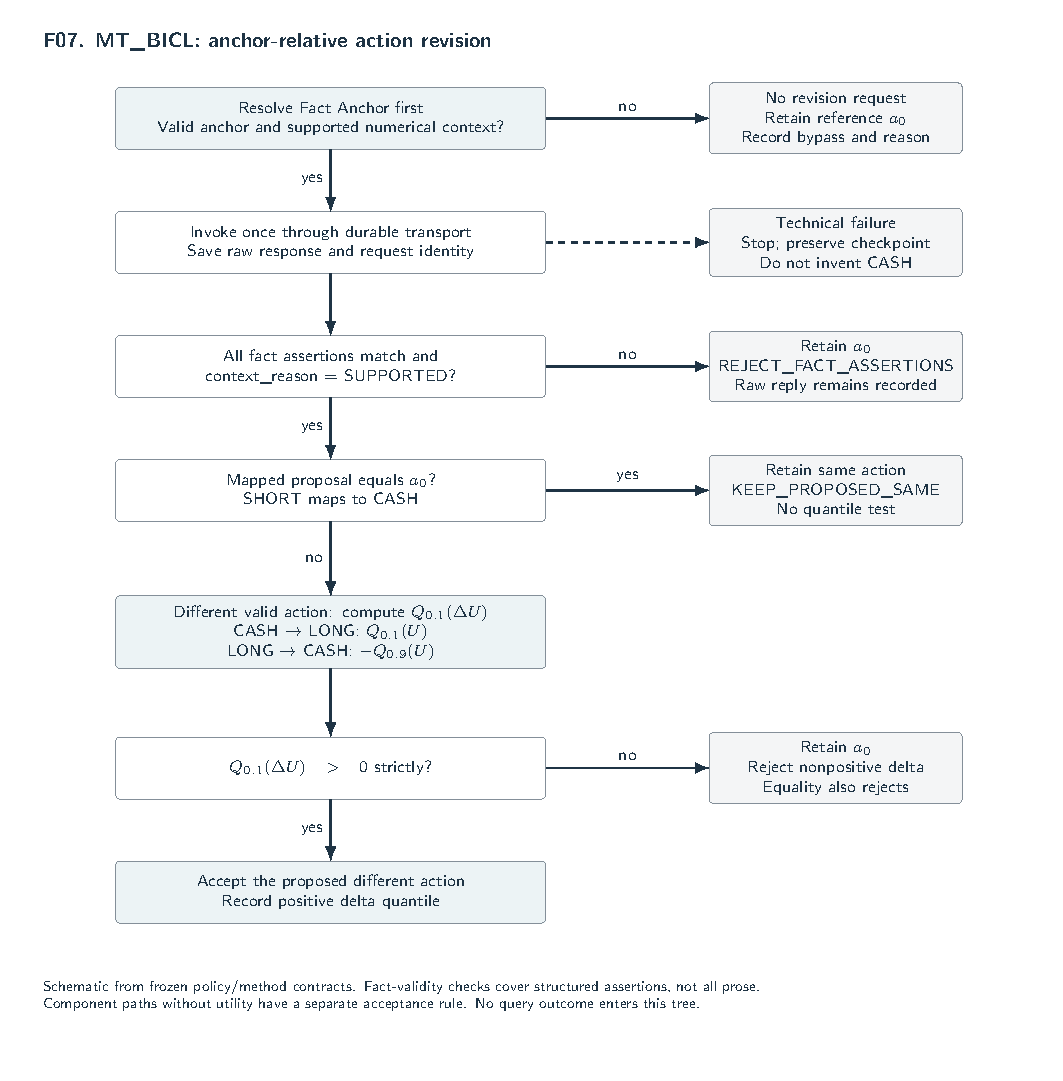
\includegraphics[width=\linewidth,height=0.72\textheight,keepaspectratio]{../assets/diagrams/F07_action_policy.pdf}
\caption{F07. Anchor-relative action revision}\label{fig:F07}\end{figure}

\textbf{Figure F07.} The implemented MT\_\allowbreak{}BICL revision path separates support
bypass, invalid response assertions, same-action retention and the strict
quantile gate. Technical errors stop execution with recoverable evidence.
The Fact Anchor is resolved before this tree. Source: BG14/BG18 and SYS33;
schematic, not measured transition frequencies.
\href{../assets/diagrams/F07_action_policy.pdf}{PDF} ·
\href{../assets/diagrams/F07_action_policy.tex}{TikZ source}.

\textbf{Illustrative gate examples, not additional research responses.} Assume
a valid anchor, supported context and a matching structured response.
All intervals below are hypothetical net-return fractions.

\begingroup
\small
\setstretch{1.05}
\setlength{\tabcolsep}{3pt}

\begin{longtable}[]{@{}
  >{\raggedright\arraybackslash}p{(\linewidth - 8\tabcolsep) * \real{0.2000}}
  >{\raggedleft\arraybackslash}p{(\linewidth - 8\tabcolsep) * \real{0.2000}}
  >{\raggedleft\arraybackslash}p{(\linewidth - 8\tabcolsep) * \real{0.2000}}
  >{\raggedleft\arraybackslash}p{(\linewidth - 8\tabcolsep) * \real{0.2000}}
  >{\raggedright\arraybackslash}p{(\linewidth - 8\tabcolsep) * \real{0.2000}}@{}}
\caption{External policy - supporting detail}\label{tab:04_proposed_system:20}\tabularnewline
\toprule\noalign{}
Anchor \ensuremath{\rightarrow} proposal
 & Q10(\(U\))
 & Q90(\(U\))
 & Q10(\(\Delta U\))
 & Result
 \\
\midrule\noalign{}
\endfirsthead
\toprule\noalign{}
Anchor \ensuremath{\rightarrow} proposal
 & Q10(\(U\))
 & Q90(\(U\))
 & Q10(\(\Delta U\))
 & Result
 \\
\midrule\noalign{}
\endhead
\bottomrule\noalign{}
\endlastfoot
CASH \ensuremath{\rightarrow} LONG & +0.002 & +0.010 & +0.002 & Accept LONG \\
CASH \ensuremath{\rightarrow} LONG & 0 & +0.010 & 0 & Retain CASH \\
LONG \ensuremath{\rightarrow} CASH & \ensuremath{-}0.012 & \ensuremath{-}0.001 & +0.001 & Accept CASH \\
LONG \ensuremath{\rightarrow} CASH & \ensuremath{-}0.012 & +0.001 & \ensuremath{-}0.001 & Retain LONG \\
\end{longtable}

\endgroup

These examples explain the rule, without generating LLM replies or
reevaluating research cases. A negative mean alone is insufficient for a
LONG\ensuremath{\rightarrow}CASH revision. EX01's raw LONG already equals anchor LONG, so its
actual reason is KEEP\_\allowbreak{}PROPOSED\_\allowbreak{}SAME and its delta-quantile field is null.
Even a hypothetical CASH proposal using that interval would fail because
Q90 is positive. EX01 therefore illustrates retention, not an observed veto.

The implemented component interventions \texttt{Plain\_\allowbreak{}revision} and \texttt{No\_\allowbreak{}utility}
omit the numeric veto: an eligible, fact-valid different action is accepted
with \texttt{NO\_\allowbreak{}NUMERIC\_\allowbreak{}VETO}. \texttt{Utility\_\allowbreak{}only} is a separate numerical comparator,
LONG iff support exists and Q10(\(U\))\textgreater0; it does not consume an LLM action.
These registered component paths are distinct from the eight roles of the
unified hosted study and must not be counted as additional unified methods.

\subsection{Traceability}\label{s:de17199a4130f6e7}

Each forecast retains a request hash, raw response/request ID, shared parent
and dependency hashes. Policy is a separate record: raw proposal, anchor,
fact validity, eligibility, bypass, reason, delta-utility quantile and final
action. A proposal of SHORT maps to CASH; the raw SHORT string remains
available. A bypass has no revision response/request ID. A completed but
invalid assertion response has raw evidence and is not a bypass.

For EX01 MT\_\allowbreak{}BICL, request \texttt{cc6bf729-\allowbreak{}784a-\allowbreak{}458a-\allowbreak{}8e40-\allowbreak{}07398fac513f} proposes
LONG. The same-repeat Fact\_\allowbreak{}Anchor proof supplies LONG; eligibility and
assertion validity are true, bypass is false, reason is
KEEP\_\allowbreak{}PROPOSED\_\allowbreak{}SAME, and final action is LONG. The anchor proof hash is
\texttt{1b4a5846\allowbreak{}92244365\allowbreak{}7bae8e91\allowbreak{}d68c7489\allowbreak{}dfd58ea9\allowbreak{}2688bdce\allowbreak{}007cb29b\allowbreak{}14f70049}.
This attributes the proposal to the hosted model and retention to policy;
it does not attribute the action to the student alone. Query prices and
labels are joined only after the forecasting barrier in Section 4.9.

\section{Variant orchestration and complete algorithms}\label{s:21530b5246fd89f6}

\subsection{Eight roles on one shared parent}\label{s:e30bc8e57ec07a81}

The unified study schedules eight roles for every point/repeat, including
Fact\_\allowbreak{}Anchor as an explicit dependency role. It does not run eight separate
upstream pipelines. One Indicator\ensuremath{\rightarrow}Pattern\ensuremath{\rightarrow}Trend realization, with the
recorded alpha/sentiment preparation, forms an immutable shared snapshot
\(u0\) for that point. Variant-specific projections use deep copies and keep
the shared parent digest. Native/Common differences in Section 4.4 remain
declared transformations of this parent, not a reason to regenerate vision.

\textbf{Table B03, complete unified-role interface.} Sections 4.4 and 4.7 provide
the foundation and four-prior deltas. This table adds execution dependencies
and the distinction between a new response and an inherited action.

\begingroup
\small
\setstretch{1.05}
\setlength{\tabcolsep}{3pt}

\begin{longtable}[]{@{}
  >{\raggedright\arraybackslash}p{(\linewidth - 6\tabcolsep) * \real{0.1800}}
  >{\raggedright\arraybackslash}p{(\linewidth - 6\tabcolsep) * \real{0.2700}}
  >{\raggedright\arraybackslash}p{(\linewidth - 6\tabcolsep) * \real{0.2800}}
  >{\raggedright\arraybackslash}p{(\linewidth - 6\tabcolsep) * \real{0.2700}}@{}}
\caption{Table B03, complete unified-role interface. Sections 4.}\label{tab:04_proposed_system:21}\tabularnewline
\toprule\noalign{}
Role / identifier
 & Added resources or context
 & Same-repeat forecast dependencies
 & No-request path / final-action rule
 \\
\midrule\noalign{}
\endfirsthead
\toprule\noalign{}
Role / identifier
 & Added resources or context
 & Same-repeat forecast dependencies
 & No-request path / final-action rule
 \\
\midrule\noalign{}
\endhead
\bottomrule\noalign{}
\endlastfoot
Native / \texttt{original\_\allowbreak{}fix} & Native report profile & None & New base reply; raw action mapped to LONG/CASH \\
Common / \texttt{original\_\allowbreak{}common} & Common report profile/instruction & None & New base reply; supplies durable fallback/reference input \\
Bayesian v1 / \texttt{bayesian\_\allowbreak{}v1} & Mature signal bank, regime, v1 prefix & Common & Retrieval fallback inherits Common; otherwise mapped reply \\
C2 & Signal bank, disjoint conditional statistics and ready examples & Common & Neither view ready: inherit Common; otherwise mapped reply \\
A / \texttt{A\_\allowbreak{}tp\_\allowbreak{}pool} & T/P conditional pool & Common & Same readiness contract; otherwise mapped reply \\
B / \texttt{B\_\allowbreak{}semantic} & C2 evidence, alternative presentation & Common & Same readiness contract; otherwise mapped reply \\
Fact Anchor / \texttt{Fact\_\allowbreak{}Anchor} & PIT numerical fact packet & Common & Completed invalid assertions select Common; missing response is an error \\
MT / \texttt{MT\_\allowbreak{}BICL} & Facts, frozen task/student resources, utility projection & Common and Fact Anchor & Ineligible/invalid anchor: retain resolved reference without revision request; otherwise apply Section 4.8.6 \\
\end{longtable}

\endgroup

\begin{figure}[htbp]\centering
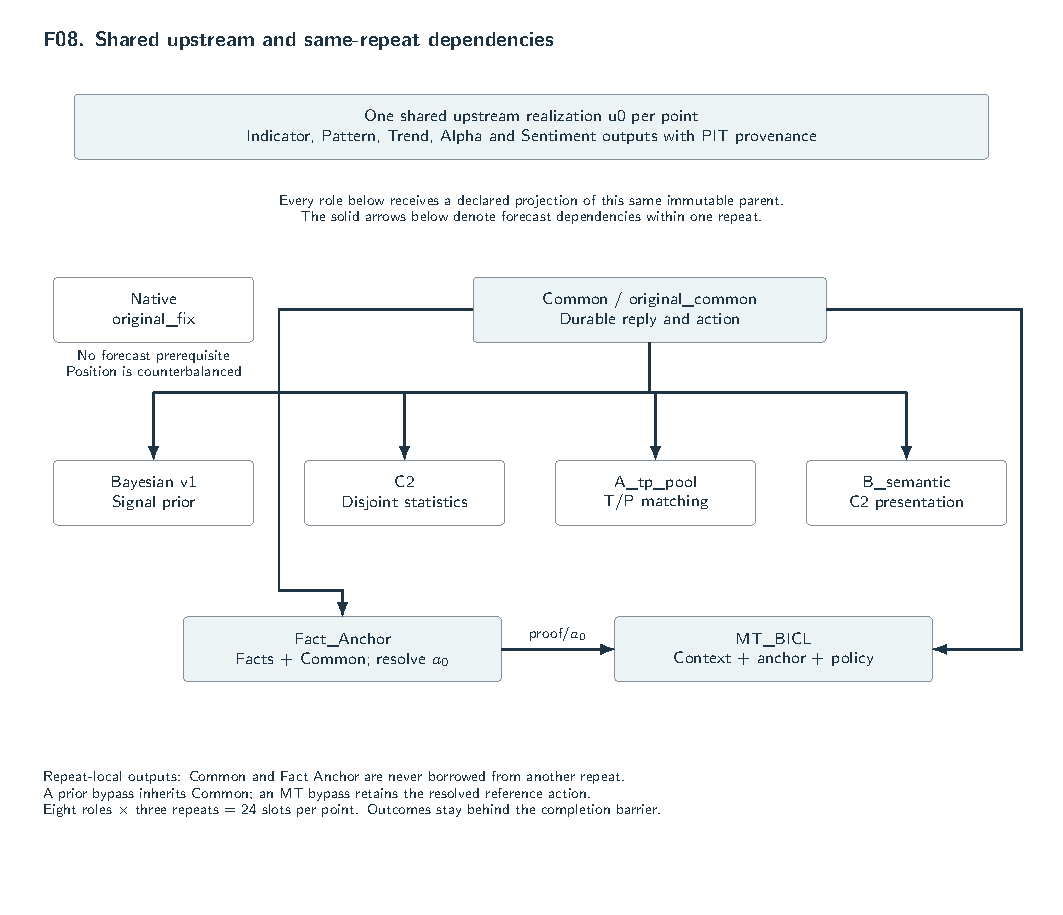
\includegraphics[width=\linewidth,height=0.72\textheight,keepaspectratio]{../assets/diagrams/F08_variant_dag.pdf}
\caption{F08. Shared parent and within-repeat dependencies}\label{fig:F08}\end{figure}

\textbf{Figure F08.} One shared upstream realization feeds eight roles; Common
and Fact Anchor are durable outputs of the same repeat. Arrows among roles
are forecast dependencies, distinct from the shared-input relation. Source:
SYS44--SYS46/BG18. This DAG specifies prerequisites rather than elapsed time
or performance. \href{../assets/diagrams/F08_variant_dag.pdf}{PDF} ·
\href{../assets/diagrams/F08_variant_dag.tex}{TikZ source}.

The runner counterbalances order subject to this DAG. For global point
index \(i\) and repeat \(r\), it uses \texttt{ordered\_\allowbreak{}branches(3i+r)}: rotate the six
Common-dependent tail priorities every eight indices, select only roles
whose dependencies are complete, and insert Native at position \((3i+r)
\bmod8\). Native has no Common prerequisite. Common always precedes its
dependents; Fact Anchor precedes MT. A dictionary of outputs is newly
created for each repeat, preventing reuse of a different repeat's Common
or anchor. A stage's parents bind the shared digest and exact dependency
output digests.\footnote{SYS44 registry, SYS45 \texttt{ordered\_\allowbreak{}branches}, SYS46 hosted runner and BG18 method adapters; CL102--CL103, ledger §9.19. The fixed research protocol has one realization/three repeats; component Full/Base remains a separate study.}

There are three Decision repeats conditional on one upstream realization.
Eight roles therefore produce 24 forecast \textbf{slots} per point, even when
some have no hosted request. A response is an actual completed model reply;
an HTTP attempt includes retries and format repair. EX01 r0 has eight
forecast slots, five Decision responses and three C2/A/B bypasses. A bypass
keeps a provenance-bearing output but adds neither a response nor a new
vision realization. Numerical controls such as always-LONG and always-CASH
are evaluated separately and are not additional hosted roles.

\subsection{Algorithms and outcome barrier}\label{s:408b36639d14b809}

The following pseudocode summarizes the frozen implementation contracts.
It describes logical operations rather than replacing the source with a
new runner. Resource fitting is a separate offline step. Smoke/control
execution does not open a research query payoff.

\hypertarget{alg:pit-context}{}

\textbf{Algorithm A01. Construct admissible historical context.}

\begin{Verbatim}[fontsize=\small,breaklines=true,breakanywhere=true]
Input: point (symbol, cutoff), registered fold/reserved IDs,
       authenticated price/news prefixes and frozen resource identities
Output: shared-input data, fact packet, signal-prior evidence,
        numerical context/utility with explicit support status
1. Validate source identity, observed calendar and horizon contract.
   Select only price rows through cutoff and admissibly dated news.
   Preserve missingness; reject invalid required inputs.
2. Construct current reports/images from the allowed analysis window.
   Retain full-source, window and report/projection identities separately.
3. For signal priors: admit same-stock mature bank episodes with exit<cutoff;
   apply the relevant regime/matching/statistics/selection/readiness rules.
   Keep population, selected and displayed counts separate.
4. For numerical tasks: use the pre-query fold pool and reserved-ID exclusion;
   enforce block/partition boundaries and strict historical exit cutoff.
   Use the frozen scaler, bucket filter and task/observation ranking.
5. Create the unlabeled query vector and numerical fact packet from PIT data.
   Validate complete membership, uniqueness, dates and source hashes.
6. Obtain frozen student probability and teacher/bootstrap utility as specified
   in Sections 4.8.3-4.8.4; record support reasons without manufacturing data.
7. Return artifacts and hashes; never attach query entry/exit prices or label.
   Required artifact/model/provenance failure raises instead of returning CASH.
\end{Verbatim}

The runner may prepare numerical resources on demand and reuse them across
repeats; A01's grouping does not imply a refit or a new stochastic upstream
call for every role. The signal-bank and numerical-context boundaries
remain different, as Section 4.5 explains.

\hypertarget{alg:method-policy}{}

\textbf{Algorithm A02. Prepare one role and resolve its final action.}

\begin{Verbatim}[fontsize=\small,breaklines=true,breakanywhere=true]
Input: shared snapshot, role, repeat, durable same-repeat dependencies
Output: durable forecast/raw/policy record
1. Validate the role/profile and prerequisite output digests.
2. Prepare a deep-copied role projection, request/schema and auxiliary proof;
   validate the final prompt budget and persist preparation before invocation.
3. If preparation prescribes no request, require raw=None:
   signal-prior fallback inherits Common; MT bypass retains resolved anchor.
4. Otherwise invoke through durable transport with the stage attempt identity;
   retain actual request/response identity and raw bytes before parsing.
   Schema repair/retry follows Section 4.10, not an action-agreement rule.
5. Resolve base action, Fact Anchor or MT revision using its declared policy.
   Keep raw proposal, validity, eligibility, bypass, reason and action separate.
6. Validate the record against request, shared parent and dependencies;
   persist completion/hash. On technical uncertainty keep the incomplete stage.
\end{Verbatim}

\hypertarget{alg:paired-evaluation}{}

\textbf{Algorithm A03. Execute paired forecasts, then join outcomes.}

\begin{Verbatim}[fontsize=\small,breaklines=true,breakanywhere=true]
Input: locked cohort, resources, run identity and three-repeat protocol
Output: completed forecasts, separate outcomes and method/account summaries
1. For each planned point, resume or create its one durable shared u0 snapshot.
2. For r=0,1,2, start an empty dependency-output map.
   Visit all eight roles in the registered counterbalanced topological order;
   run/resume A02 and put each complete output in that repeat's map.
3. Require all 24 forecast slots complete and validated for the point.
   Only then invoke the research outcome oracle and persist its separate stage.
   Smoke/control stages retain an explicit no-query-payoff marker instead.
4. Join saved final LONG/CASH actions to the canonical LONG payoff and net label.
   Preserve source identity, units, fixed Open(t+1)/Close(t+3) and two-way costs.
5. Rebuild chronological accounts separately by method/repeat/symbol/fold,
   validating nonoverlap and the registered support before compounding.
6. Compute classification, account and paired summaries on their defined units;
   distinguish forecast slots from distinct market points and accounts.
\end{Verbatim}

The logical barrier prevents outcome access during this forecasting run.
It does not erase previous donor-data exposure or prove that the entire
study is a previously untouched causal holdout. The Native row-wise audit
FAIL and whole-system NOT\_\allowbreak{}CERTIFIED limitations remain those of the locked
evidence. Pairing controls current upstream variation; it does not remove
all uncertainty or isolate the student from the rest of the pipeline.
\footnote{BG16/BG17 providers, SYS46 hosted barrier and SYS47 outcome/evaluation functions; CL104--CL105. A01--A03 are source-bound pseudocode, not newly executed algorithms. EX01 validation reads timestamps/dependency hashes from the archive only.}

For EX01 the archived outcome stage lists the 24 required slots. Each
forecast/prepare stage is complete before the outcome starts, with Common
and anchor dependencies matching the corresponding repeat's output hash.
Section 4.10 returns to these records to explain recovery and the final
outcome, without putting that outcome in A01 or the hosted prompt.

\section{Prompt limits, recovery and application}\label{s:052b7113d7072810}

\subsection{Prompt admission and bounded repair}\label{s:ce26cfc79aae04ca}

\hyperref[s:3c1d039c39c73d45]{Appendix B} supplies request IDs, measured examples, explicitly labeled English presentation translations and compact reply schemas for these prompt families.

Report compression is part of the model's input contract. \texttt{\_\allowbreak{}distill\_\allowbreak{}report}
selects summaries according to report type: alpha keeps its numerical
summary, sentiment removes the article-list/prose section, and Indicator
prefers its convergence summary when the recognized heading exists.
\texttt{\_\allowbreak{}cap\_\allowbreak{}report} then retains roughly 70\% of the available character budget
from the head and the rest from the tail, with a visible truncation marker.
If a heading is not recognized, the cap can remove informative middle
content; Section 4.3's EX01 example records this limitation rather than
assuming the full report reached Decision.

\begingroup
\small
\setstretch{1.05}
\setlength{\tabcolsep}{3pt}

\begin{longtable}[]{@{}
  >{\raggedright\arraybackslash}p{(\linewidth - 4\tabcolsep) * \real{0.2400}}
  >{\raggedleft\arraybackslash}p{(\linewidth - 4\tabcolsep) * \real{0.3900}}
  >{\raggedleft\arraybackslash}p{(\linewidth - 4\tabcolsep) * \real{0.3700}}@{}}
\caption{Prompt admission and bounded repair - supporting detail}\label{tab:04_proposed_system:22}\tabularnewline
\toprule\noalign{}
Report
 & Backtest cap (characters)
 & General live cap (characters)
 \\
\midrule\noalign{}
\endfirsthead
\toprule\noalign{}
Report
 & Backtest cap (characters)
 & General live cap (characters)
 \\
\midrule\noalign{}
\endhead
\bottomrule\noalign{}
\endlastfoot
Trend & 800 & 900 \\
Pattern & 800 & 900 \\
Indicator & 800 & 900 \\
Alpha & 1,100 & 1,200 \\
Sentiment & 500 & 600 \\
\end{longtable}

\endgroup

Common-based study requests use the backtest limits. The live column
describes a separate default cap dictionary, not evidence that a serving
variant may ignore its own final guard. Prefixes are bounded at 600,
the fact card at 700 and the anchor card at 80. The final assembled text,
including instructions, reports, separators and the response example,
must have \textbf{fewer than 6,500 characters}. The unified adapter checks again
after adding the Common instruction and causal source card. A format-repair
suffix also passes a final length check. Overflow fails before dispatch;
it does not trigger removal of historical members or a weaker schema.
These are character limits, not token counts. Transport separately reserves
estimated request/output tokens and applies quota admission.\footnote{SYS02 distill/cap/guard, SYS18/SYS42/BG18 assembly, SYS52 final length guard and SYS48 repair admission; CL106, ledger §9.20. Live UI presentation differs from the frozen Decision byte identity as declared in §3 of the ledger.}

\subsection{One retry owner and durable HTTP evidence}\label{s:51de81f6c5f8a255}

Agent invocation goes through \texttt{\_\allowbreak{}invoke\_\allowbreak{}with\_\allowbreak{}retry}. In a research invocation
scope it delegates one attempt to \texttt{invoke\_\allowbreak{}once}, leaving retry ownership
to the durable transport. Nested agent/SDK retry loops must not multiply
the execution budget; the recorded request sets SDK retries to zero.
The legacy unscoped wrapper has its own bounded retry loop and caps its
delay at 60 seconds; it must not be described as the hosted runner's
complete recovery policy.

In the unified durable path, each active logical execution has at most three
HTTP attempts in total, including transient failures, confirmed NOT\_\allowbreak{}SENT
attempts and Decision schema repair. Ordinary resume preserves this count;
the explicitly authorized replacement generations below are separate. For
HTTP 429/500/502/503/504, the transport computes the next eligible time
from the maximum of capped exponential backoff \(\min(900,5\,2^j)\),
\texttt{retry-\allowbreak{}after}, and a parsed \texttt{retry after X s} response message. Header/body
waits are not truncated to the exponential term's cap. The schedule is
reconstructed from persisted raw evidence after interruption.

A 200 response is persisted before JSON/schema parsing. An invalid
Decision JSON/schema may request the fixed format-repair suffix within
the same total attempt budget. A vision parse failure does not silently
regenerate the image interpretation. Semantic disagreement, low confidence,
an unwanted action, or a schema-valid mismatch with facts is not a format
repair criterion. Such a mismatch reaches the explicit policy in Section
4.8.6. Unsupported context bypasses before transport and consumes no
request attempt.\footnote{SYS48 \texttt{DurableCalls.\allowbreak{}call/\allowbreak{}cooldown/\allowbreak{}ready}, SYS49 invocation scope, SYS02 wrapper and frozen U08 transport; CL107--CL108. Standalone legacy retry and durable research recovery are different paths.}

\textbf{Versioned admission, not one timeless quota rule.} U08 began with pooled
per-organization accounting across models, rolling windows, carried usage
and provider headers. From HTTP sequence 487 the locked amendment uses
\texttt{per\_\allowbreak{}org\_\allowbreak{}model\_\allowbreak{}v1}, separating admission buckets by organization/model.
From sequence 591 it uses \texttt{provider\_\allowbreak{}response\_\allowbreak{}v1}: admission follows actual
provider transient-error cooldown for that organization/model, not local
count windows or successful-response remaining headers. Request-budget and
phase-attempt caps remain. These are zero-based sequence boundaries recorded
in the runtime manifests, not newly inferred provider entitlements.
Deferral yields a future eligible time; exhaustion or an ambiguous send
retains evidence and blocks that execution.
The cooperative runner can continue other ready queues while preserving
the fixed assignment of each point. Historical quota settings are not a
claim about the provider's current limits or an instruction to collect
new data.

\subsection{Checkpoint lifecycle and recovery}\label{s:158597603efd21d7}

The run identity binds the source/protocol/runtime/resource inputs and run
UUID. A deterministic slot name identifies point, realization, repeat and
role. \texttt{StageBook} checkpoints render/graph/shared, preparation, forecast
and outcome stages; durable transport separately checkpoints each HTTP
intent and raw response. Each stage retains inputs, parent digests,
attempt UUID, status, output and output digest in an atomic envelope.
Completion is validated before it can satisfy a dependency or the outcome
barrier.\footnote{SYS50 \texttt{StageBook}, SYS51 journal save/load, SYS48 HTTP evidence/reconciliation and SYS46 hosted barrier; CL109. This section describes source contracts and reads existing EX01 records; no recovery execution is newly claimed.}

\begingroup
\small
\setstretch{1.05}
\setlength{\tabcolsep}{3pt}

\begin{longtable}[]{@{}
  >{\raggedright\arraybackslash}p{(\linewidth - 4\tabcolsep) * \real{0.2400}}
  >{\raggedright\arraybackslash}p{(\linewidth - 4\tabcolsep) * \real{0.3900}}
  >{\raggedright\arraybackslash}p{(\linewidth - 4\tabcolsep) * \real{0.3700}}@{}}
\caption{Checkpoint lifecycle and recovery - supporting detail}\label{tab:04_proposed_system:23}\tabularnewline
\toprule\noalign{}
State or interruption
 & Recovery behavior
 & What must remain separate
 \\
\midrule\noalign{}
\endfirsthead
\toprule\noalign{}
State or interruption
 & Recovery behavior
 & What must remain separate
 \\
\midrule\noalign{}
\endhead
\bottomrule\noalign{}
\endlastfoot
Stage complete and hashes valid & Return the validated saved output; no new model call & Reuse within the same identity versus a fresh repeat response \\
Preparation complete, forecast not complete & Resume the forecast with the same stage identity and transport history & Prepared request versus completed reply \\
HTTP 200 raw durable, stage completion interrupted & Parse/validate that saved response, then complete the stage & Local reconstruction versus a new HTTP request \\
Transient response durable & Honor persisted cooldown/quota and remaining attempt budget & Deferral versus valid policy bypass \\
HTTP intent UNKNOWN after possible send & Stop automatic dispatch for that UUID; reconcile delivery evidence & Unknown delivery versus missing statistical support \\
Confirmed not sent & Record NOT\_\allowbreak{}SENT with evidence; retain history/reservation and consumed attempt & Reconciliation versus resetting the attempt cap \\
Corrupt envelope, changed request/parent/run identity & Raise; do not reuse the output under altered inputs & Integrity failure versus an ordinary resume \\
\end{longtable}

\endgroup

UNKNOWN is written before sending because a process can fail after the
provider receives the request but before the response is durably saved.
It is unsafe to infer from a missing local response that no call occurred.
\texttt{reconcile\_\allowbreak{}not\_\allowbreak{}sent} requires an explicit unique UUID and evidence; it does
not mark an uncertain response as successful. The stage wrapper may reenter
an incomplete local callback under the same attempt, but transport refuses
to resend an unresolved UNKNOWN. It reuses a validated raw 200 instead.
The hosted path does not use the older generic journal reconciliation to
invent a new stage UUID and reset HTTP accounting.

\textbf{Recorded replacements are explicit exceptions to ordinary resume.}
The frozen run includes user-authorized replacement generations for
VCB-2026-04-01 and VJC-2025-12-19, and a later replacement of the exhausted
\texttt{forecast/\allowbreak{}VCB-\allowbreak{}2026-\allowbreak{}09-\allowbreak{}23/\allowbreak{}u0/\allowbreak{}r2/\allowbreak{}MT\_\allowbreak{}BICL} slot. The manifests bind backups,
retired HTTP digests, affected stages and preserved completed outputs.
The point replacements can regenerate affected upstream stages under a
new generation; the single-slot replacement retains its shared preparation.
The final retirement map contains 15 old HTTP records. They remain in
the complete ledger and phase cost/attempt accounting, while active
forecast verification uses the replacement generation. A valid completed
response may not be retired merely to seek a preferred action. This is
neither automatic UNKNOWN replay nor an invisible reset of scientific
history. Pairing refers to each point's accepted shared parent; it does
not imply that no failed generation ever existed.\footnote{SYS53--SYS57 model/provider admission and point/slot replacement contracts; U08 frozen runtime manifests OP01--OP04, ledger §9.20; CL110. Sequence boundaries, targets and retired counts come from the archived manifests. No replacement is performed while writing this chapter.}

These rules give three distinct point lifecycles. A successful point saves
shared input, all preparations and forecasts, then opens the outcome.
A support-limited point still completes a provenance-bearing inherited
action for the affected slot, with no fake request, and can cross the
barrier when all roles finish. An interrupted point remains incomplete
until delivery/integrity is resolved; its missing slot keeps the outcome
closed. A receipt cannot count the third lifecycle as a valid CASH
forecast merely to reach the planned sample size.

EX01's saved stages illustrate the completed lifecycle and three prior
bypasses, not a new interruption experiment. The UNKNOWN/recovery rows
above describe source-defined behavior; writing them does not dispatch a
request, simulate a crash or rerun a cold acceptance test. The application
workflow and final EX01 outcome follow in the next two subsections.

\subsection{Application workflow and interpretation}\label{s:f9572fb99dc08a53}

\hyperref[s:cc9510fc96476c9d]{Appendix F} gives the source-checked entrypoints and resource requirements, separating offline fixtures, historical cold replay and provider-backed live analysis.

The Flask application exposes the method through a \textbf{Realtime 1D analysis
form}. A user selects a stock and one of six main versions: Original,
Bayesian v1, C2, A, B or MT-BICL, then starts analysis. The current form
does not expose an as-of source selector, comparison/repeat controls or
multiple timeframes. Backend capabilities and earlier UI modes must not
be mistaken for controls on this form. Original delegates to the legacy
analysis route; enhanced versions use a captured live snapshot, preflight
and one analysis job with one repeat.\footnote{AP01 contract, AP03 registry, AP04--AP11 live capture/provider/runtime and AP13--AP15 form sources, pinned separately from the research snapshot in ledger §9.21; CL111--CL113. Current form and older/backend daily-closed capabilities are explicitly distinguished.}

For an enhanced selection, the client captures \texttt{\{symbol,timeframe:\allowbreak{}"1d"\}},
validates the returned snapshot identity and submits the same locked
selection to preflight and job creation. The current form uses the
versioned timeframe envelope even for 1D. It is distinct from the backend's
older \textbf{latest completed daily session} capture, which excludes today's
bar before 15:30 local time. The current timeframe path may include a
forming daily observation and records \texttt{daily\_\allowbreak{}provisional}. During the
session it can extend daily context from observed intraday stock/index
data; outside the session it uses the available daily index calendar.
Provisional data are not silently described as an exchange-certified close.

The capture validates positive/consistent OHLCV, timestamps, source freshness,
at least 600 daily stock/index observations, matching cutoff and calendar
membership. It preserves the chart separately from the daily context and
rejects future timestamps or inconsistent units. News without publication
dates is excluded; future publication is rejected. Date-only publication
is admitted conservatively from the following day. Insufficient verified
scores remain unavailable, not neutral. The snapshot records source,
capture time, units, provisional status and vendor/corporate-action limits.
It is hashed and bound to the owner before forecasting.

Preflight verifies resources, supported domain, request/model/options and
dependency plan. Selecting MT schedules Common\ensuremath{\rightarrow}Fact Anchor\ensuremath{\rightarrow}MT for that
point/repeat; it does not schedule all eight study roles or three research
repeats. The requested version, executed dependencies and an inherited
fallback action remain distinguishable. Job identity binds the capture,
configuration, model/prompt/resource versions and owner scope; secrets stay
on the server. Reload/resume reads the old capture under its hash. Newer
market data require a new capture/job, rather than altering an existing
job's source midway.

\begin{figure}[htbp]\centering
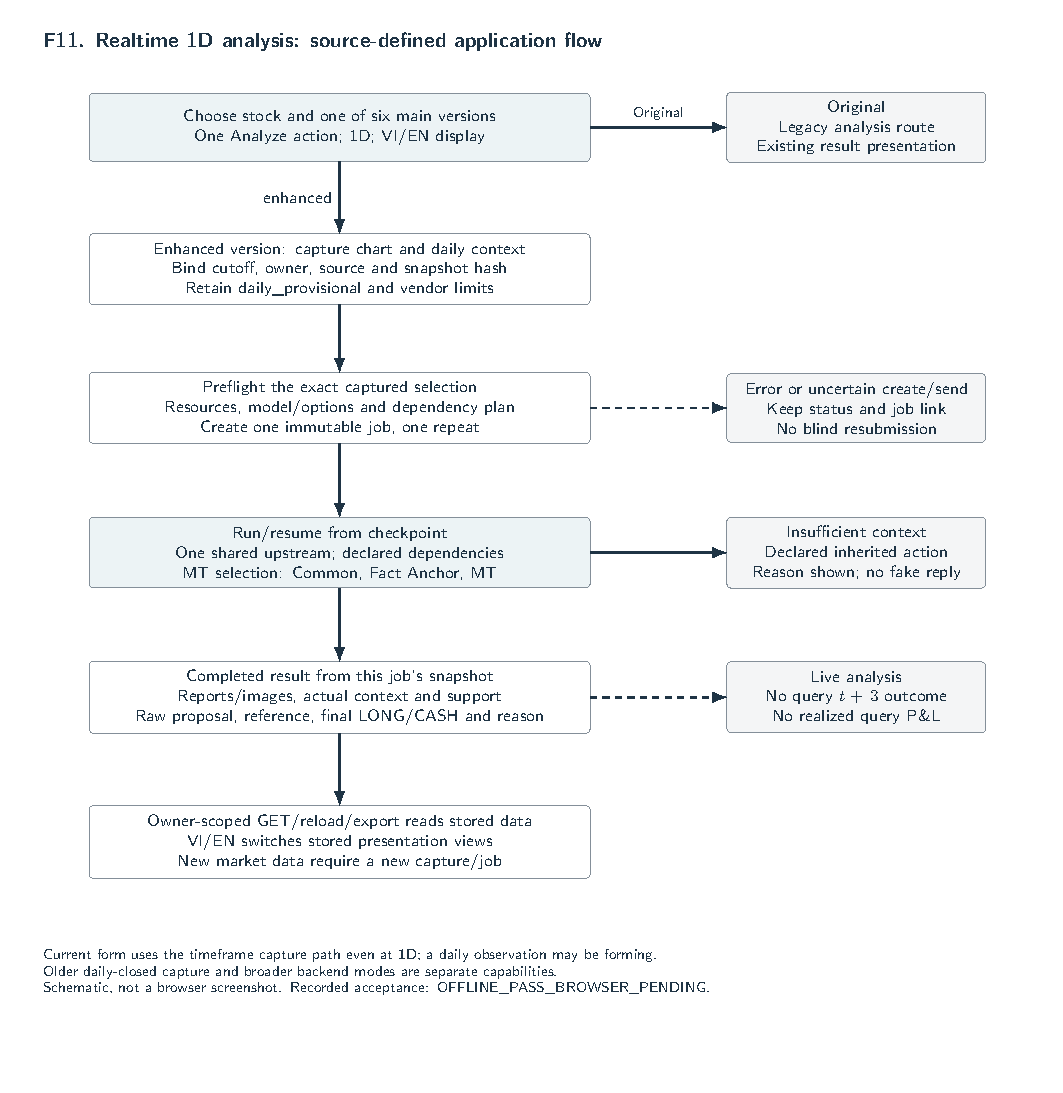
\includegraphics[width=\linewidth,height=0.72\textheight,keepaspectratio]{../assets/diagrams/F11_application_flow.pdf}
\caption{F11. Application analysis workflow}\label{fig:F11}\end{figure}

\textbf{Figure F11.} Source-defined Realtime 1D workflow with a legacy Original
branch and a snapshot-bound enhanced branch. The result is read from the
same job; an uncertain create/send is not automatically repeated. This is
an explanatory schematic, not a screenshot or browser acceptance result.
Source: application bindings AP01--AP15 in the ledger.
\href{../assets/diagrams/F11_application_flow.pdf}{PDF} ·
\href{../assets/diagrams/F11_application_flow.tex}{TikZ source}.

\textbf{Frozen resources applied to a new query.} Enhanced live inference reuses
the historical bank, feature scaler, HMM and student weights. Common alpha
transfers the frozen top-five selection/orientations/threshold to the new
price prefix under \texttt{live\_\allowbreak{}frozen\_\allowbreak{}selector\_\allowbreak{}transfer\_\allowbreak{}v1}; it does not refit
the selector on the query. MT historical labels remain frozen before
1 July 2026. Historical facts keep the label source; only query features
and facts use the captured live data. Planned weekday \(t+1/t+3\) metadata
do not supply future prices or a verified exchange settlement calendar.
The target remains daily Open(\(t+1\))\ensuremath{\rightarrow}Close(\(t+3\)), not three intraday bars.
The live vendor transfer and unavailable independent corporate-action
ledger remain scientific limitations.

\textbf{Progress and result reading.} The overlay follows checkpointed agent
progress, including dependency/context work; it does not rerun agents for
animation. Completed enhanced jobs open the result page with a live-source
job identifier. Reports and images come from that job's checked snapshot,
not global images or a previous session. The BICL panel explains actual
context/support, reference\ensuremath{\rightarrow}final action and bypass/rejection reasons before
the final Decision display. Native alpha and Common alpha are labeled
separately because the upgraded Decision input is not the native report.

Interpret raw proposal as the model's output, final LONG/CASH as the policy
action, and null metrics as unavailable/pending. A support bypass explains
inheritance; a failed or UNKNOWN job is not a completed CASH forecast.
An ambiguous create response disables blind resubmission and retains the
job link when available. GET/export/reload read recorded results without
market capture or model inference. The enhanced live analyze path has no
query outcome or realized \(t+3\) P\&L; a stated confidence/R:R is not such an
outcome.

The current presentation profile \texttt{live\_\allowbreak{}bilingual\_\allowbreak{}presentation\_\allowbreak{}v1} stores
VI/EN views with the job. Pattern/Trend and Decision obtain presentation
text within their existing invocation; canonical fields alone feed policy.
Numerical report labels use deterministic localization. Changing the
display language reads stored views and does not send a translation
request or change the canonical forecast. This presentation contract has
its own wire identity: the author's accepted equivalence of the live
modules' research logic does not mean their raw source/request bytes are
identical to the historical snapshot.\footnote{AP02 output route, AP12 presentation mixin, AP16 receipt and AP17 QA archive; CL114/CL116. The archived checks, source bindings and pending browser status are inspected without opening an application session or rerunning tests.}

The recorded application receipt is \textbf{OFFLINE\_\allowbreak{}PASS\_\allowbreak{}BROWSER\_\allowbreak{}PENDING} with
\texttt{f11\_\allowbreak{}complete=false}; desktop/mobile visual acceptance has not run.
It reports 135 Python and 24 DOM checks, with Python evidence reused under
source bindings and the documented DOM delta, rather than claiming every
check ran again after every edit. These are recorded fixture/scoped checks,
not newly executed tests here, live fills, prospective validation or proof
of profitable deployment. No UI screenshot is presented as accepted. The
diagram and workflow text let the method be understood while preserving
this outstanding acceptance boundary.

\subsection{Closing EX01 after the forecasting barrier}\label{s:0a3a61d80b3973e9}

Return to FPT at the 3 July 2023 cutoff. Its 600-bar shared prefix contains
the 45-bar analysis window; sentiment is unavailable. Pattern's low
confidence/warning and Trend's interpretation remain recorded observations,
not independently verified chart truth. The signal-prior regime is
CONSOLIDATION, while the separately sourced MT regime is BULL. These labels
are not edited to match. V1 supplies three signal examples; C2/A/B fail
readiness and inherit Common. MT uses three prior tasks and three target
observations, 14 labeled historical rows in total, with the query unlabeled.

The saved r0 actions complete the walkthrough before outcome access:

\begingroup
\small
\setstretch{1.05}
\setlength{\tabcolsep}{3pt}

\begin{longtable}[]{@{}
  >{\raggedright\arraybackslash}p{(\linewidth - 6\tabcolsep) * \real{0.1800}}
  >{\raggedright\arraybackslash}p{(\linewidth - 6\tabcolsep) * \real{0.2700}}
  >{\raggedright\arraybackslash}p{(\linewidth - 6\tabcolsep) * \real{0.2800}}
  >{\raggedright\arraybackslash}p{(\linewidth - 6\tabcolsep) * \real{0.2700}}@{}}
\caption{Closing EX01 after the forecasting barrier - supporting detail}\label{tab:04_proposed_system:24}\tabularnewline
\toprule\noalign{}
Role
 & Raw proposal
 & Final action
 & Recorded resolution
 \\
\midrule\noalign{}
\endfirsthead
\toprule\noalign{}
Role
 & Raw proposal
 & Final action
 & Recorded resolution
 \\
\midrule\noalign{}
\endhead
\bottomrule\noalign{}
\endlastfoot
Native & SHORT & CASH & RAW\_\allowbreak{}DECISION \\
Common & LONG & LONG & RAW\_\allowbreak{}DECISION \\
Bayesian v1 & LONG & LONG & RAW\_\allowbreak{}DECISION \\
C2 & None & LONG & FALLBACK\_\allowbreak{}ORIGINAL \\
A & None & LONG & FALLBACK\_\allowbreak{}ORIGINAL \\
B & None & LONG & FALLBACK\_\allowbreak{}ORIGINAL \\
Fact Anchor & LONG & LONG & NO\_\allowbreak{}NUMERIC\_\allowbreak{}VETO \\
MT-BICL & LONG & LONG & KEEP\_\allowbreak{}PROPOSED\_\allowbreak{}SAME \\
\end{longtable}

\endgroup

The five raw replies and three bypass outputs refer to the same upstream
realization, but their role-specific requests are different. Across all
three repeats, every required slot is durable before the outcome stage
starts. \textbf{Only after that barrier} does the separate EX01 outcome record
expose entry Open on 4 July and exit Close on 6 July, with 5 July the middle
session. Entry is VND 48,180 and exit VND 48,390, after the declared unit
conversion from the source series.

The canonical oracle gives

\[
r^{\mathrm{net}}=\frac{48{,}390}{48{,}180}
 \frac{(1-0.001)(1-0.0025)}{(1+0.001)(1+0.0025)}-1
=-0.00264731712420041.
\]

Gross return is +0.4358655044\%, but net return is \textbf{\ensuremath{-}0.2647317124\%} and the
economic label is DOWN. Each LONG action receives that one-cycle loss;
Native's CASH receives zero under the stated comparator contract, without
opening a short position. This does not establish that Native is superior
over the study, or that a negative estimated mean forced MT's action.
EX01 intentionally retains an incorrect net-label LONG decision rather
than replacing it with a winning illustration.\footnote{EX01 U08 shared/prepared/raw/policy/outcome members in ledger §7 and §9.21; TIME01 canonical oracle and TIME06 source identity; CL115. Numbers and timestamps are read from locked records; no historical model call or portfolio evaluation is rerun.}

Account returns require the full chronological sequence of nonoverlapping
cycles and the registered account/repeat aggregation. This single payoff
is not the study's portfolio return. Entry/exit prices, realized return and
net label remain in the evaluation record, outside the earlier reports,
context, projection and model requests. The chapter has followed one
decision from admissible inputs through agents, historical context and
policy to its later economic outcome; Chapter 5 evaluates those decisions
on the locked cohorts and reports the limitations of the two studies.
